%%=============================================================================
%% Methodologie
%%=============================================================================

\chapter{\IfLanguageName{dutch}{Methodologie}{Methodology}}
\label{ch:methodologie}

%% TODO: Hoe ben je te werk gegaan? Verdeel je onderzoek in grote fasen, en
%% licht in elke fase toe welke stappen je gevolgd hebt. Verantwoord waarom je
%% op deze manier te werk gegaan bent. Je moet kunnen aantonen dat je de best
%% mogelijke manier toegepast hebt om een antwoord te vinden op de
%% onderzoeksvraag.

Technologische details zoals performantie en energiezuinigheid worden quasi irrelevant wanneer professionals en studenten niet in staat zijn om de softwaretools te gebruiken die ze nodig hebben voor hun dagelijkse taken. Opdat professionals en studenten bereid zouden zijn om over te stappen naar een laptop of desktop die gebruik maakt van de ARM architectuur, moeten de gebruiksvriendelijkheid en software ondersteuning gelijkwaardig zijn aan die van het x86-platform. Het is niet ongewoon dat ontwikkelaars problemen en onregelmatigheden ondervinden bij het gebruik van bepaalde softwarepakketten, IDE’s of enigszins verouderde programmeertalen. Gewone computergebruikers zijn echter niet vertrouwd met soortgelijke problemen die hun werkstroom kunnen onderbreken. Vandaar dat het essentieel is voor ARM computers om een stabiele en verfijnde gebruikerservaring te voorzien voor gewone computergebruikers. ICT professionals zijn vertrouwd met het aanpassen en sleutelen van software zodat deze een ervaring biedt die perfect is afgestemd op hun eigen unieke gebruikssituatie. Dit gezegd zijnde is het uiteraard essentieel dat hun taken zonder al te veel problemen en onderbrekingen worden uitgevoerd en voltooid.

Dit onderdeel van de studie is gericht op het onderzoeken van de software compatibiliteit en het gebruiksgemak van ARM-gebaseerde desktop-besturingssystemen. Scenario 1 is gericht op alledaags gebruik zoals browsen en kantoorsoftware. In scenario 2 komen de geavanceerde ICT toepassingen aan bod die deel uitmaken van het dagelijkse softwarepakket van een student toegepaste informatica of een ICT professional.

Het is uiteraard onmogelijk om elke vorm van computergebruik te onderzoeken, vandaar dat elke gekozen toepassing bij de scenario’s gepaard zal gaan met een verklaring omtrent de relevantie ervan.

Deze praktische opstellingen zullen uitgevoerd worden aan de hand van twee toestellen. Het eerste apparaat is een Raspberry Pi 4 die beschikt over een quad core Cortex-A72 (ARM v8) 64-bit SoC en 4GB LPDDR4-3200 SDRAM \autocite{Pi2021}. Dit toestel maakt gebruik van Raspberry Pi OS, voorheen bekend als \textit{Raspbian}. Deze Linuxdistributie maakt deel uit van de \textit{Debian} familie en is grotendeels gebaseerd op de populaire Ubuntu \textit{distro}. Raspberry Pi OS is echter sterk geoptimaliseerd en gespecialiseerd voor de familie van Raspberry Pi toestellen die gebruikmaken van ARM processoren. Het voornaamste verschil met andere Linuxdistributies is de relatief eenvoudige LXDE desktopomgeving die is aangepast om minder resources te verbruiken \autocite{Pi2011}.

Het tweede apparaat dat deel uitmaakt van deze studie is een 13‑inch MacBook Pro die is uitgerust met een M1 \textit{Apple Silicon} processor. Dit toestel zal gebruikt worden om de gebruikerservaring en de software ondersteuning te testen op het macOS (ARM) platform. Bij het ontwikkelen van deze nieuwe processorarchitectuur heeft Apple ernaar gestreefd om een desktopervaring te bieden die evenwaardig is aan of beter dan het huidige macOS x86-64 platform \autocite{Apple2020}. Dit onderzoek zal deze gedurfde marketing beweringen uiteraard in vraag stellen en testen.

Om het Windows 11 on ARM besturingssysteem te testen zal deze research gebruikmaken van een virtuele opstelling door middel van Parallels Desktop 17. Deze versie van de bekende virtualisatiesoftware ondersteunt de \textit{Apple Silicon} architectuur en voorziet een goede integratie tussen het host- en gevirtualiseerde systeem. Deze werkwijze gaat echter wel gepaard met een bepaald percentage aan prestatieverlies en enkele eigenaardigheden, echter in het kader van dit onderzoek zal deze virtuele benadering volstaan.

\begin{figure}[h]
	\centering
	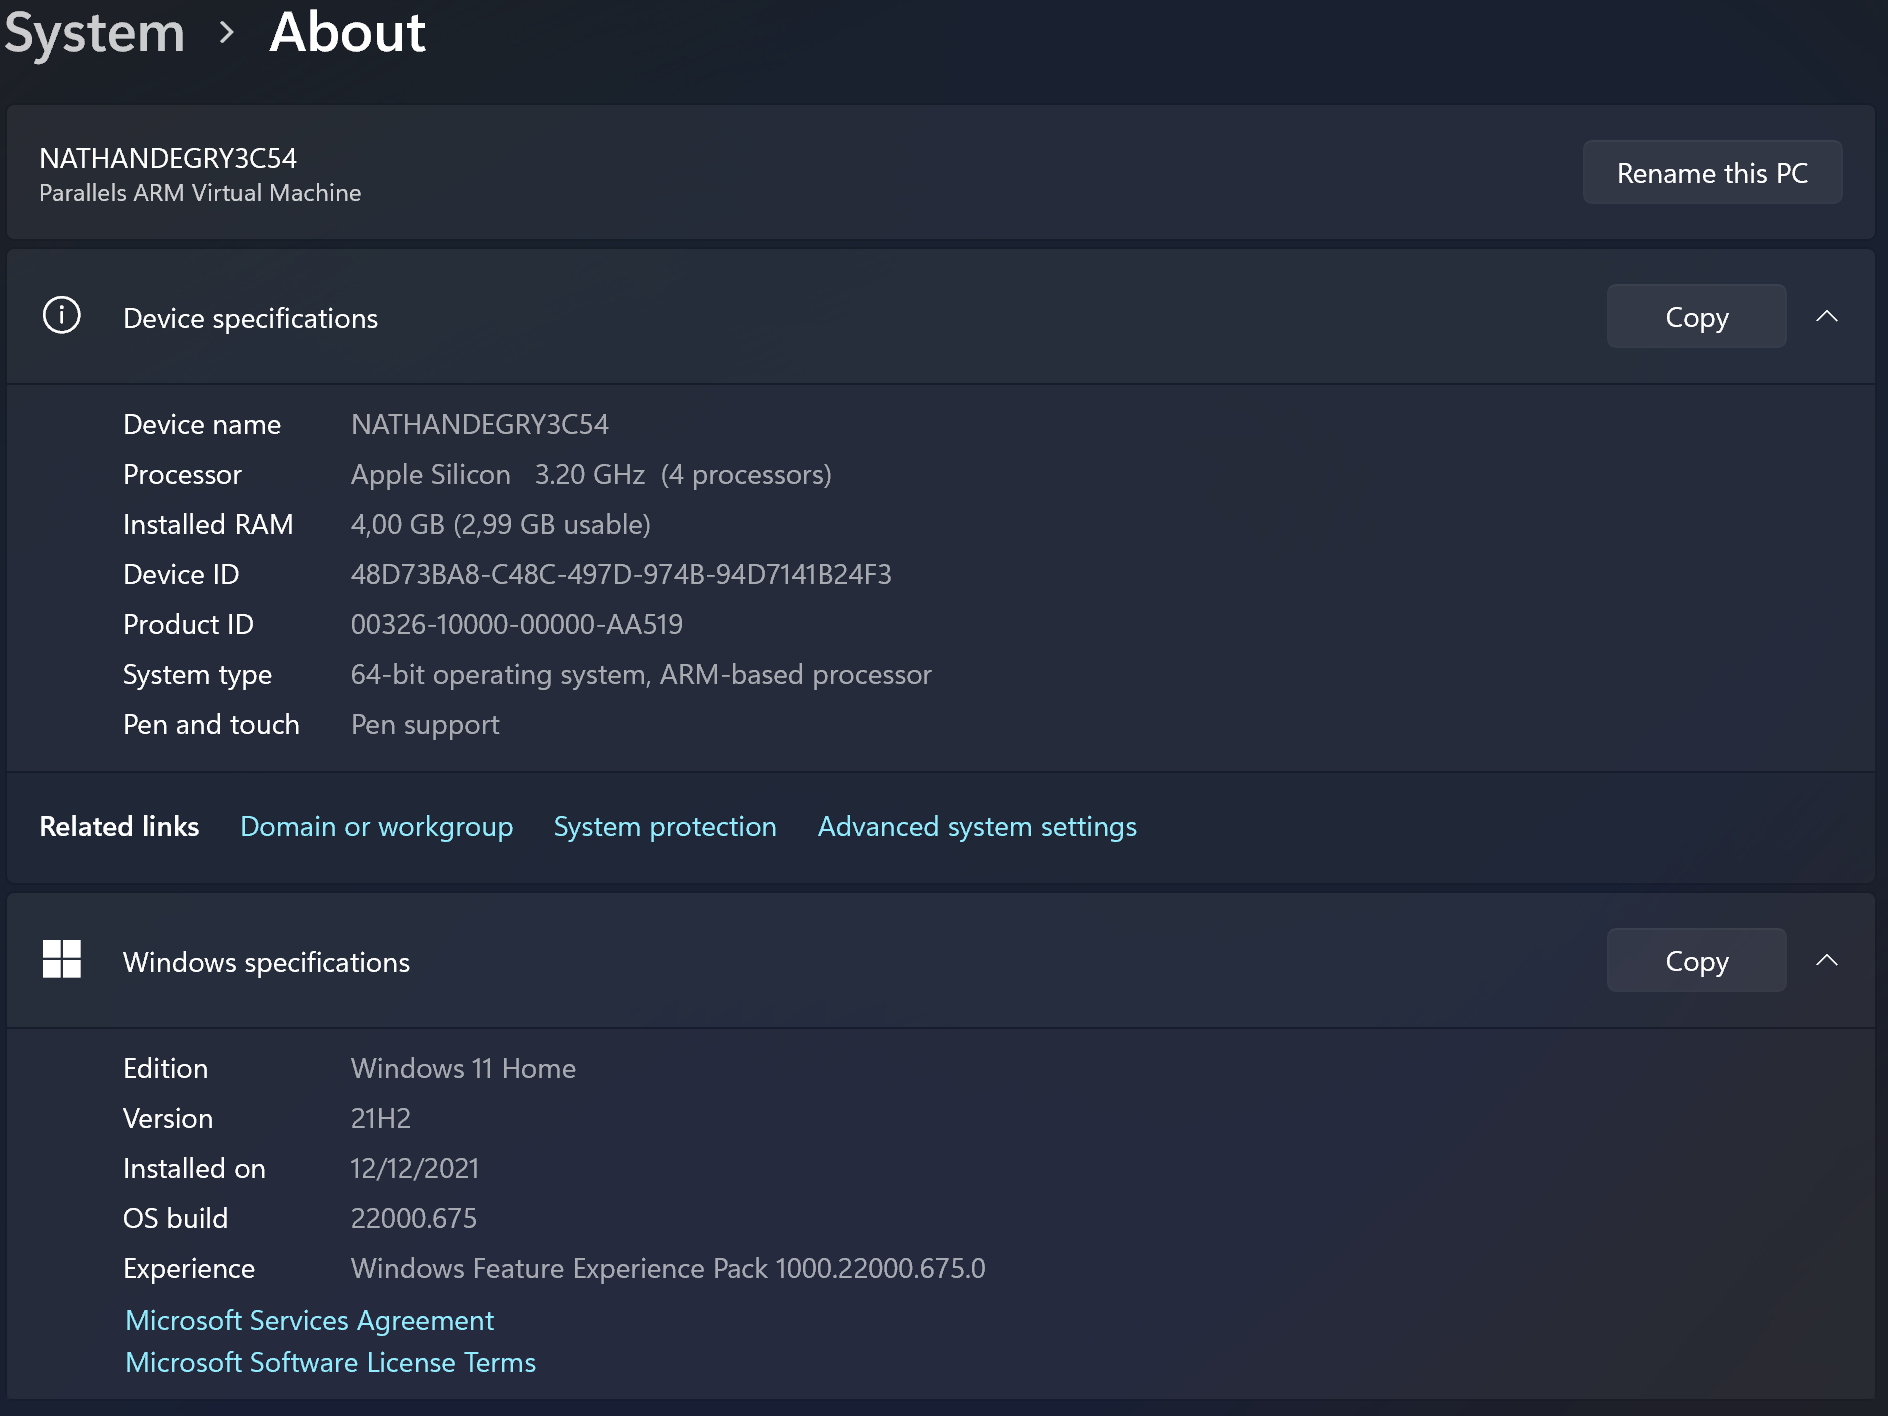
\includegraphics[width=100mm, scale=0.5]{img/specificaties_winARM.png}
	\caption{Specificaties van het gevirtualiseerde systeem Windows 11 on ARM systeem}
	\end{figure}

\newpage
\section{Scenario 1: alledaags gebruik}
Dit eerste scenario omvat software die vrijwel ondenkbaar is bij hedendaagse kantoorjobs en bachelor/master opleidingen. Een studie gevoerd door \textcite{Braganza2022} bracht aan het licht dat browsers gebaseerd op de Chromium \textit{engine}, Microsoft Office en Slack veruit de meest gebruikte applicaties zijn door professionals met een kantoorjob. Indien laptops en desktops met ARM processoren willen doorbreken bij het grote publiek, is het essentieel dat deze programma’s een gebruikerservaring aanbieden die niet te onderscheiden is van deze op x86 toestellen.

\subsubsection{Raspberry Pi OS}
Microsoft Office is tot op de dag van vandaag nog steeds veruit de meest populaire office suite. Deze populariteit kan verklaard worden door de dominantie in de onderwijs- en businessmarkt. Ondanks deze populariteit is Microsoft Office niet beschikbaar op Linux gebaseerde besturingssystemen. In dit scenario is de keuze tussen een x86 of een ARM systeem dus irrelevant. Desondanks dit opvallend tekort zijn Linux computers niet afgeschreven voor kantoorgebruik. LibreOffice is sinds jaar en dag een uitstekende optie voor gebruikers die niet wensen te betalen voor een Office 365 abonnement of een eenmalige aankoop van Microsoft Office. LibreOffice valt onder de noemer van de opensourcesoftware en is bijgevolg gratis voor de eindgebruiker. Sommigen zullen de grafische gebruikersomgeving wat verouderd en rudimentair vinden, maar verder biedt dit softwarepakket een gebruikerservaring die evenwaardig is met andere office software. Indien een gebruiker zou overschakelen naar LibreOffice, moet deze aanvankelijk bereid zijn om sommige taken opnieuw te leren, maar na een korte transitieperiode zou hij/zij geen verdere tekortkomingen of problemen mogen ondervinden. Dit gezegd zijnde, is niet elk bedrijf bereid om Microsoft Office aan de kant te schuiven voor een ander product louter op basis van het feit dat het merendeel van de medewerkers vertrouwd zijn met de Microsoft variant. Indien een gebruiker toch wenst gebruik te maken van Microsoft Office, dan is dit mogelijk via de browser. Deze variant biedt echter niet dezelfde functionaliteit als de desktop variant, maar voor alledaags gebruik zou deze moeten volstaan.

\begin{figure}[!h]
	\centering
	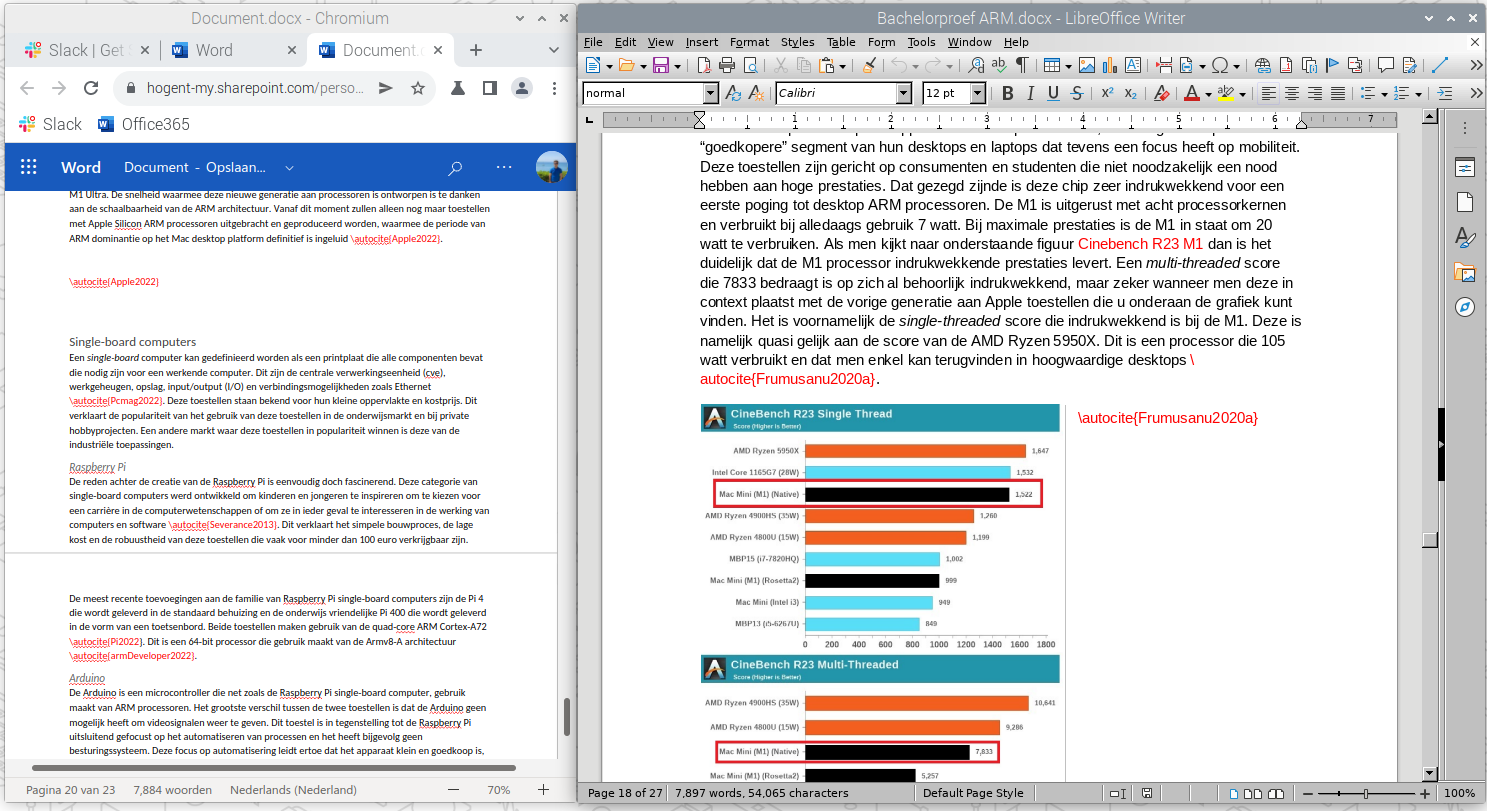
\includegraphics[width=110mm, scale=0.7]{img/office_pi.png}
	\caption{LibreOffice en Office 365 op de Raspberry Pi 4}
\end{figure}

\newpage
Slack is het communicatiemiddel bij uitstek in de bedrijfswereld en is vandaar uiteraard essentieel bij een moderne kantoorjob. Deze tool wordt integraal ondersteund op x86 Linux besturingssystemen, maar is echter opvallend afwezig op Raspberry Pi OS. Een mogelijke oplossing voor dit tekort is het gebruiken van Slack in de Chromium browser, maar dit is voor velen geen kwalitatief alternatief.

\begin{figure}[!h]
	\centering
	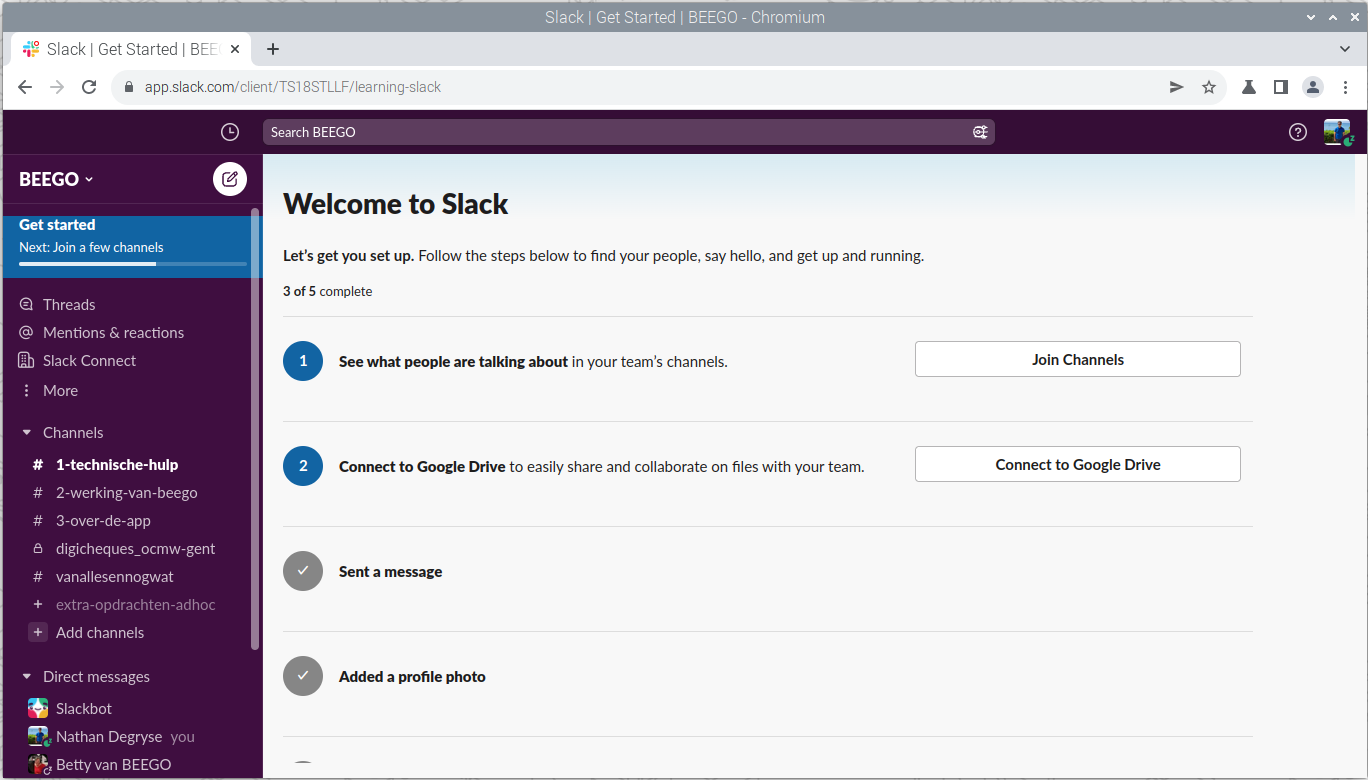
\includegraphics[width=110mm, scale=0.7]{img/slack_pi.png}
	\caption{Slack op de Raspberry Pi 4}
\end{figure}

Chromium is de standaardbrowser op het Raspberry Pi OS besturingssysteem. Dit is een open source variant van de Google Chrome webbrowser die gericht is op eenvoud, stabiliteit en performantie \autocite{ChromiumProject2009}. Een van de grootste nadelen die komt bij het gebruik van Chromium is dat het geen integratie met Google services ondersteunt. Een gebruiker kan bijvoorbeeld een account aanmaken, maar dit is enkel een lokaal account. Het is bijgevolg niet mogelijk om in te loggen op een werk- of privé Google-account waar men bladwijzers, data of andere instellingen kan importeren. Verder zijn de populaire Google Chrome en Microsoft Edge browsers niet ondersteund op Linux besturingssystemen die uitgevoerd worden op een ARM processor. Mozilla’s Firefox webbrowser is het enige volwaardige alternatief voor Chromium.

\subsubsection{macOS Monterey Apple Silicon}
De situatie verbetert aanzienlijk wanneer er wordt overgeschakeld naar macOS Monterey op een \textit{Apple Silicon} toestel. Zoals eerder werd aangehaald, verstrekte Apple enkele maanden voor de officiële release van hun nieuwe architectuur een \textit{Developer Transition Kit} (DTK). Dit toestel gaf ontwikkelaars de mogelijkheid om hun bestaande software of hun nieuwe projecten te hercompileren zodat ze een \textit{native} versie konden aanbieden \autocite{Apple2020}. Deze aanpak lijkt grotendeels succesvol te zijn geweest aangezien alle te testen applicaties in dit scenario \textit{native} verkrijgbaar zijn en een gebruikerservaring aanbieden die niet te onderscheiden is van macOS Monterey die draait op een x86 systeem.

Slack en alle Microsoft Office applicaties afgezien van Microsoft Teams, zijn vrij te verkrijgen in de App Store. Microsoft Teams dient gedownload te worden via de browser, dit is echter ook het geval bij de x86 variant van macOS Monterey. Een eindgebruiker heeft als het ware geen idee dat zijn/haar applicaties actief zijn op een systeem dat gebruik maakt van een processorarchitectuur die verschillend is van hetgeen waar hij/zij tot dan toe vertrouwd mee was. Naast het betaalde Microsoft Office pakket stelt Apple hun iWork suite gratis beschikbaar voor iedereen die een \textit{Apple ID} heeft. Dit softwarepakket is geen volwaardig alternatief voor Microsoft Office, maar ze biedt voldoende mogelijkheden voor gewone eindgebruikers en studenten.

\begin{figure}[!h]
	\centering
	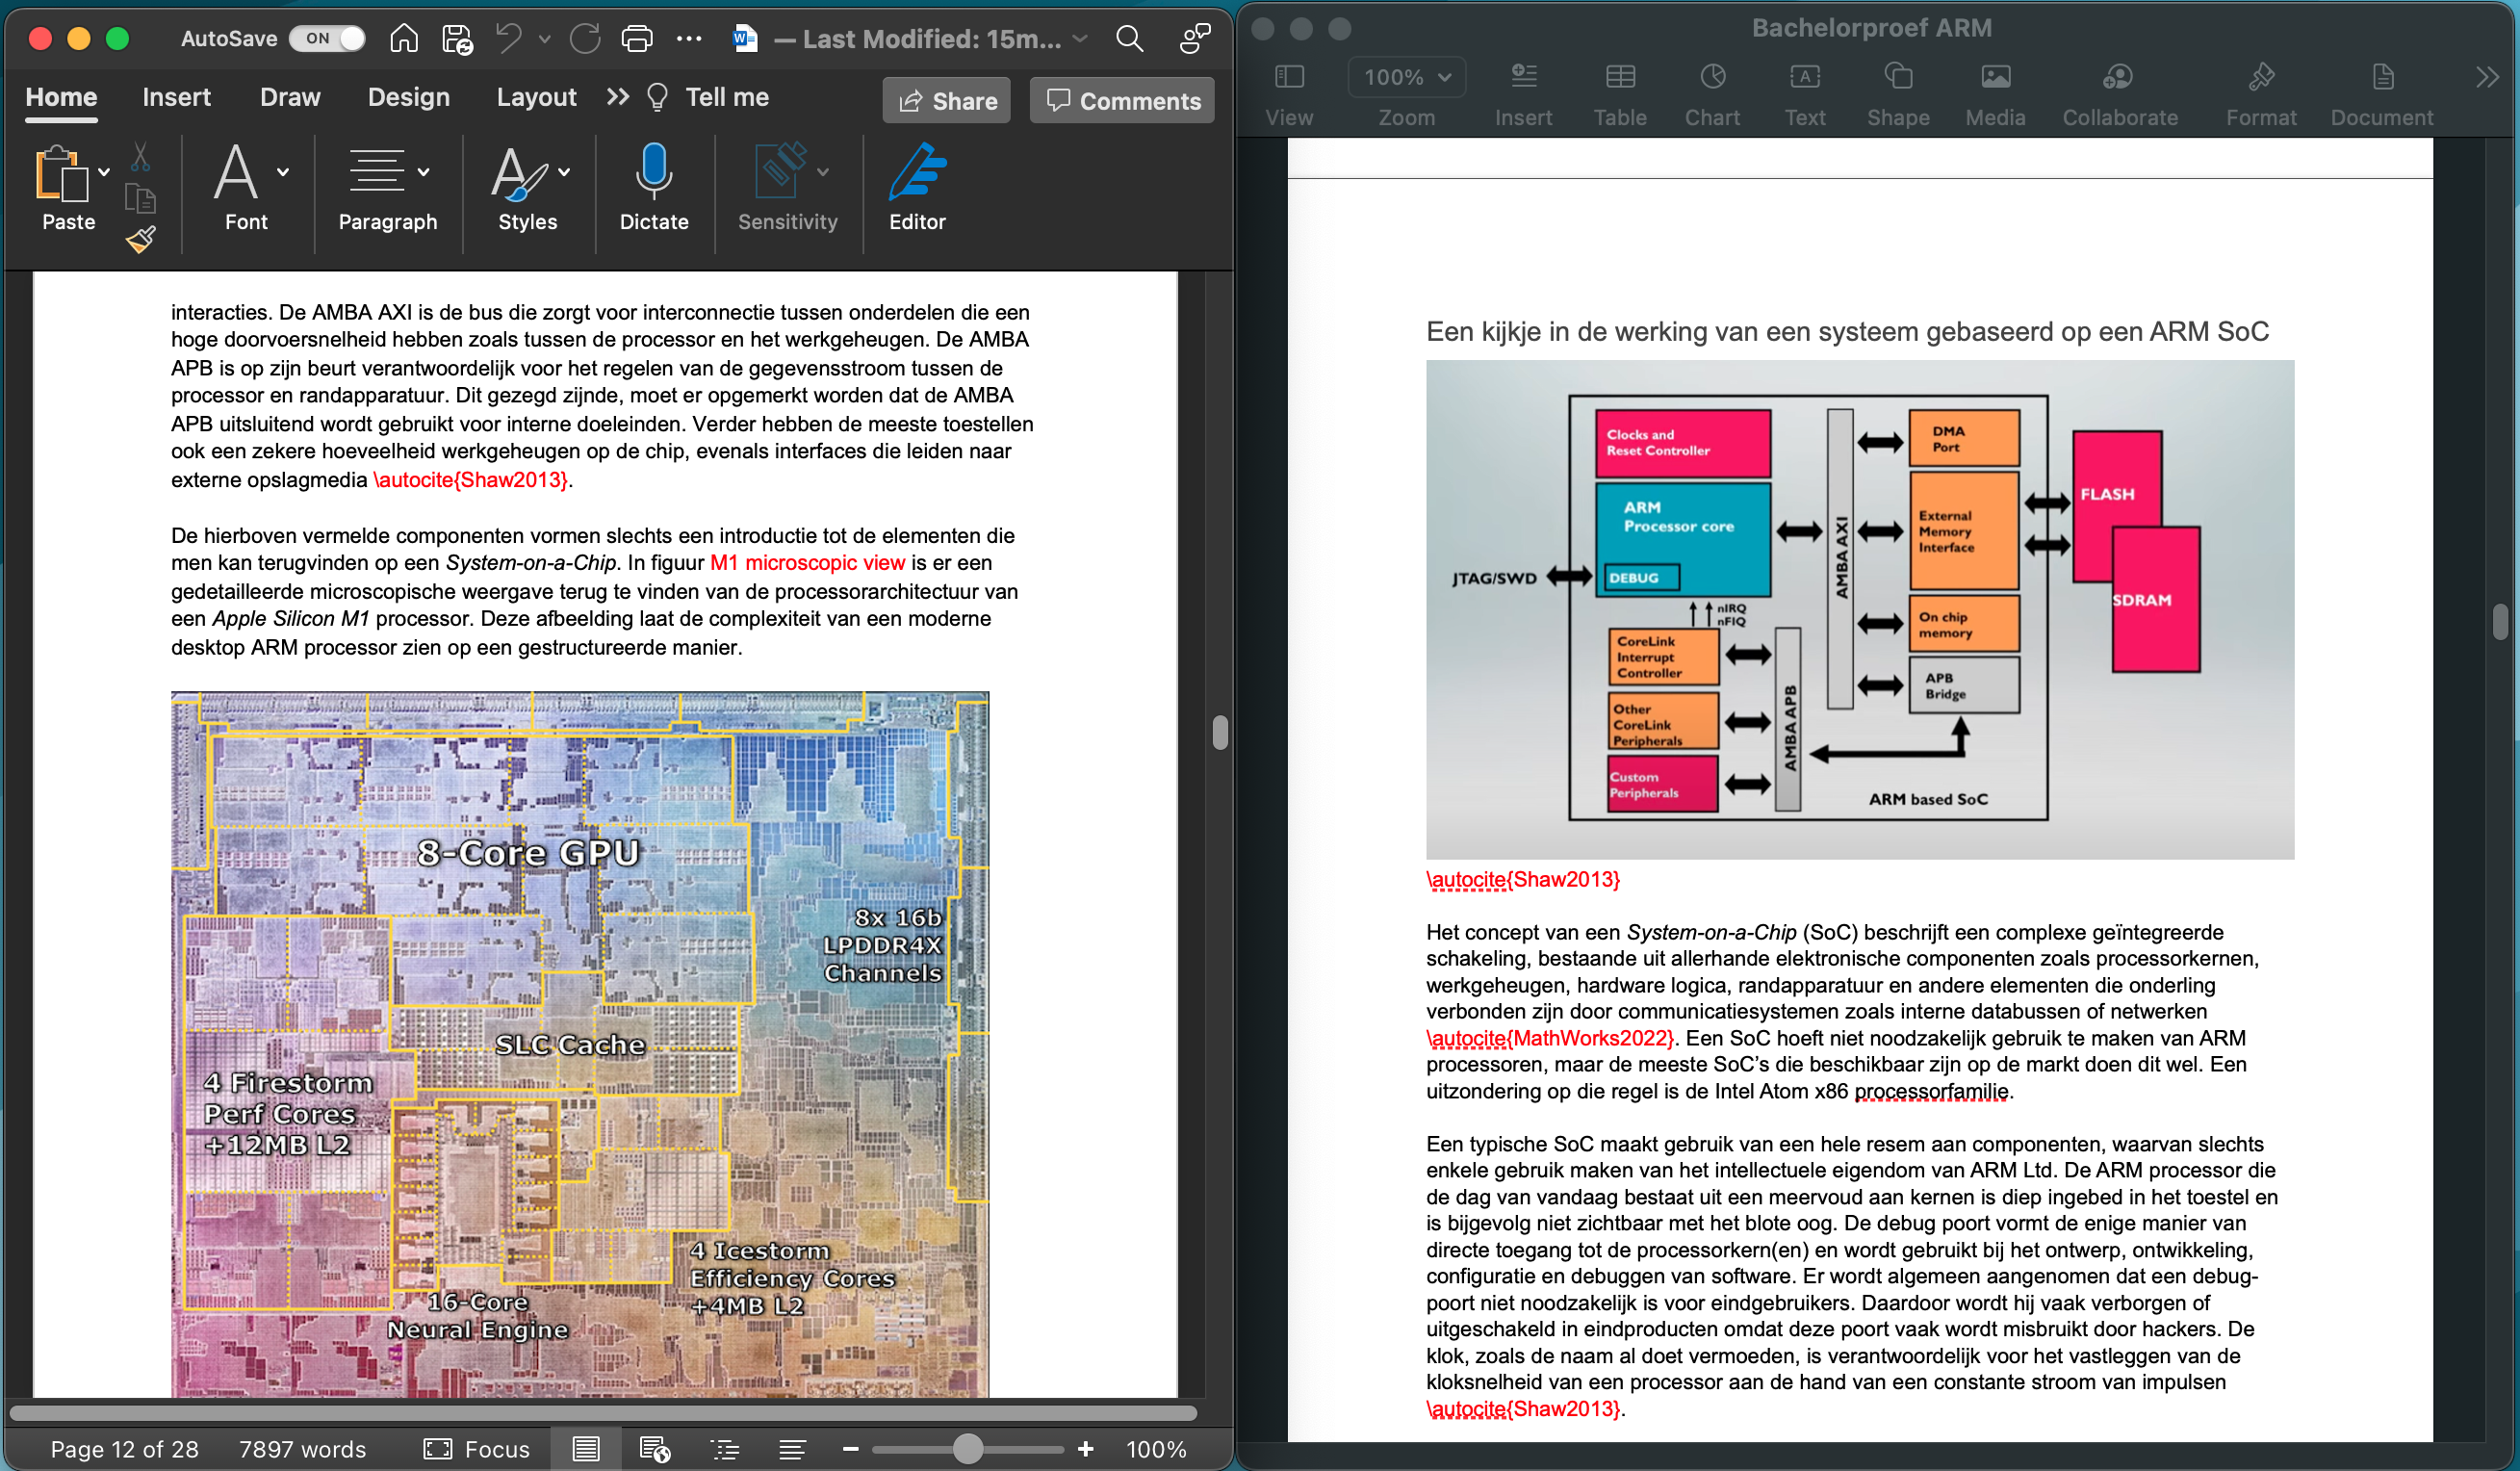
\includegraphics[width=110mm, scale=0.7]{img/office_macOSM1.png}
	\caption{Pages en Microsoft Word op het Apple Silicon platform}
\end{figure}

De enige manier waarop een eindgebruiker te weten kan komen of een applicatie gecompileerd is voor de Apple Silicon architectuur of gebruikmaakt van de Rosetta 2 \textit{translation layer} is de activiteitenweergave applicatie. Deze biedt een handig overzicht van de gebruikte processorarchitectuur in de \textit{kind} kolom. In het onderstaande voorbeeld is er te zien dat Microsoft OneDrive en WhatsApp nog niet \textit{native} ondersteund zijn.

\begin{figure}[!h]
	\centering
	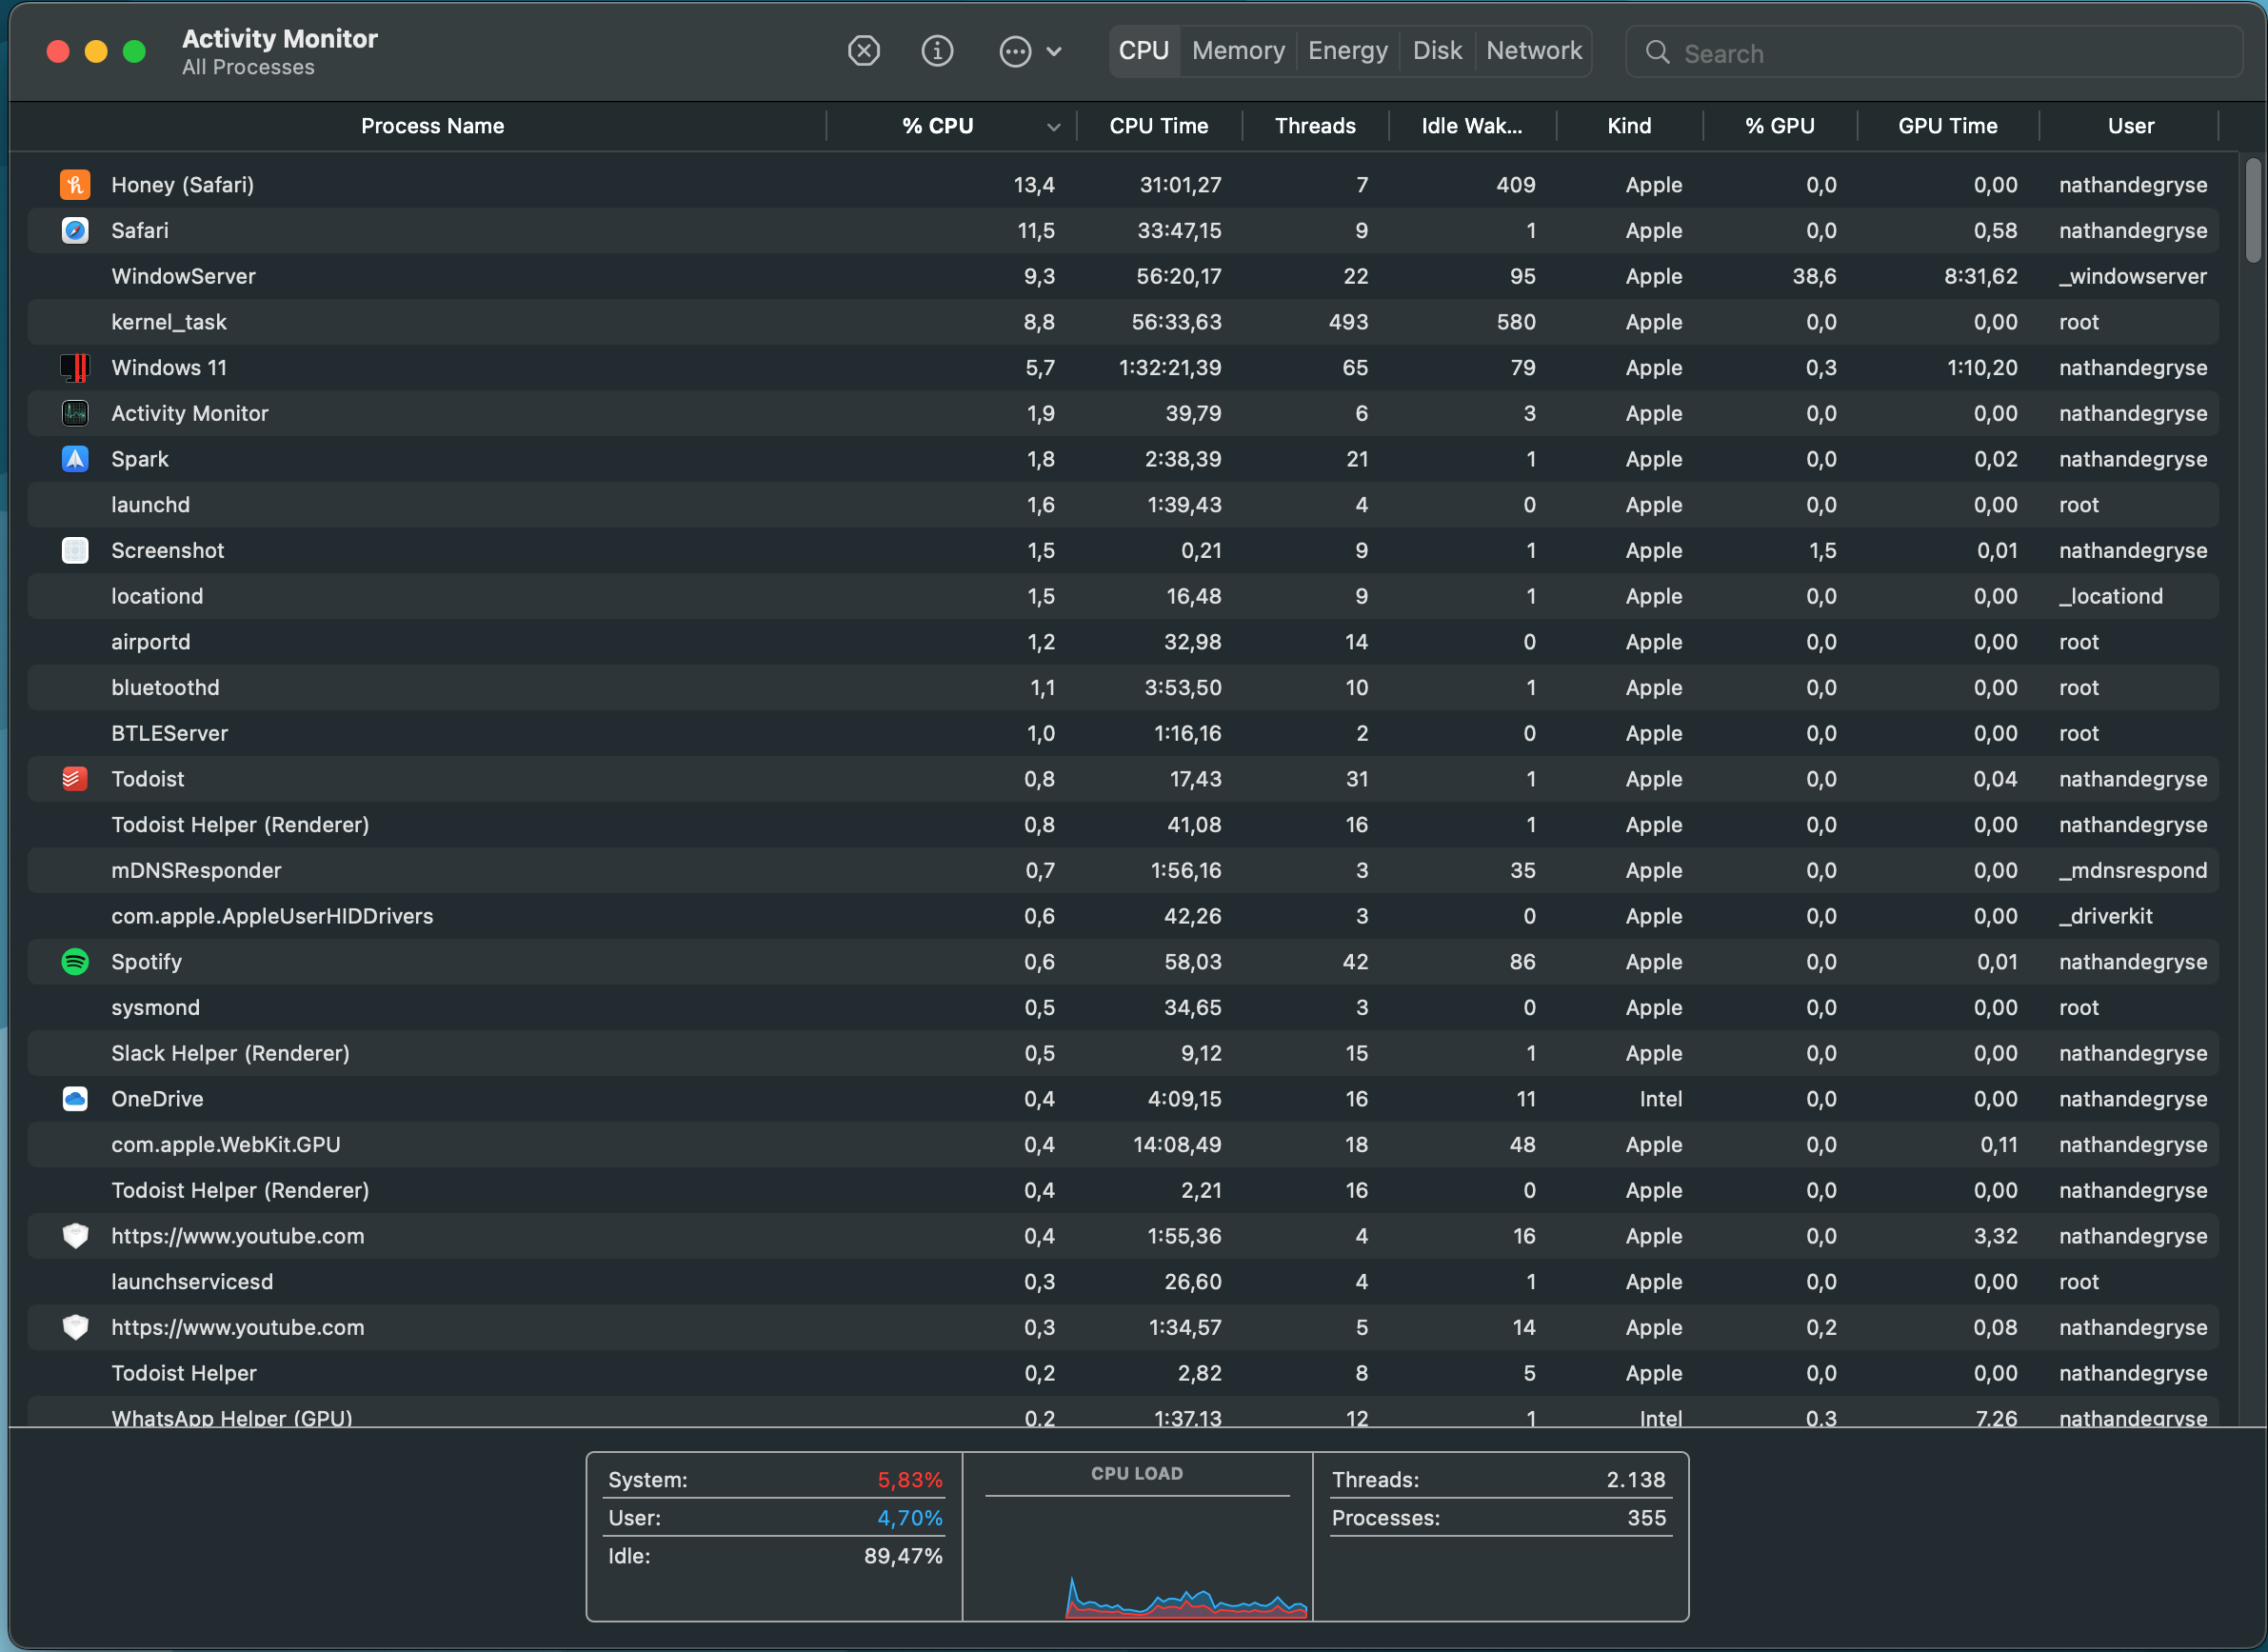
\includegraphics[width=110mm, scale=0.7]{img/activitymonitor_macOSM1.png}
	\caption{Een overzicht van de activiteitenweergave applicatie}
\end{figure}

Wat webbrowsers betreft is er geen tekort aan opties op macOS. Google Chrome, Microsoft Edge, Mozilla Firefox, Brave enzovoort worden allemaal ondersteund op het \textit{Apple Silicon} platform. Wanneer een gebruiker een browser naar keuze wenst te downloaden, krijgt deze een dialoogvenster te zien waar hij/zij kan kiezen tussen de Intel x86 variant of de versie die gericht is op het \textit{Apple Silicon} platform.

\begin{figure}[!h]
	\centering
	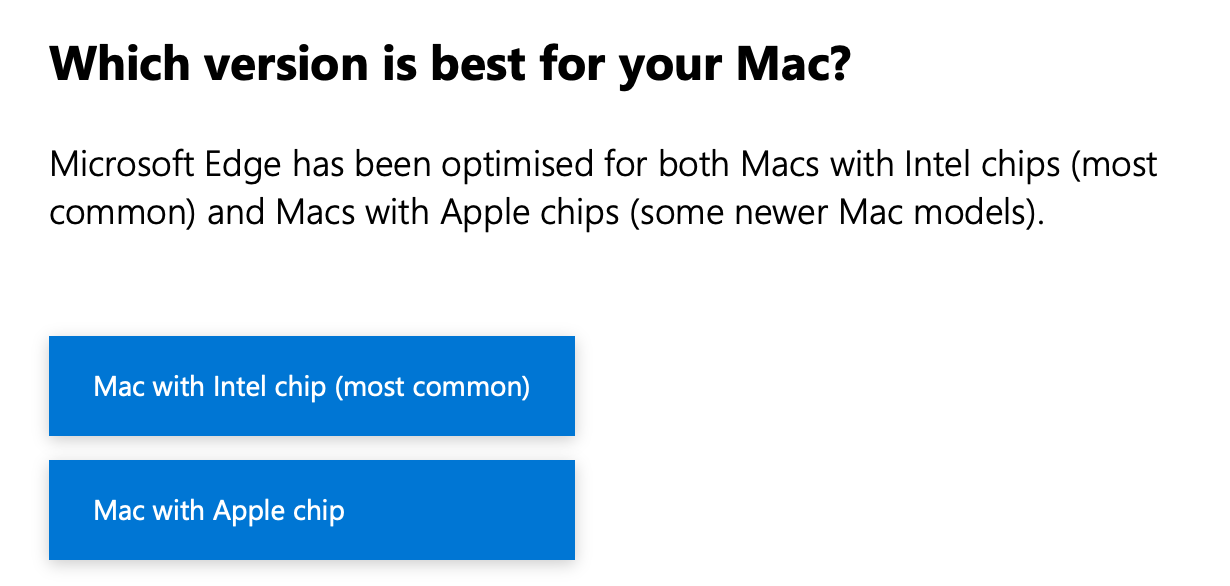
\includegraphics[width=110mm, scale=0.7]{img/browserversie_macOSM1.png}
	\caption{De Microsoft Edge download pagina \autocite{Microsoft2022}}
\end{figure}

\subsubsection{Windows 11 on ARM}
Net als op macOS voor de \textit{Apple Silicon} architectuur, zijn de meeste native Windows 11 on ARM applicaties verkrijgbaar via de appstore die gericht is op het eigen platform, in dit geval is dit de Microsoft Store die voorheen bekend stond als de Windows Store. Slack heeft een \textit{native} versie die compatibel is met Windows 10 en Windows 11 on ARM en deze bevat alle toepassingen die aanwezig zijn op het Slack communicatieplatform.

Microsoft Office heeft ook een native Windows on ARM versie, deze is echter vreemd genoeg niet terug te vinden in de Microsoft Store. Een gebruiker dient deze te downloaden via de Office 365 portaalsite. Verder krijgt een gebruiker geen indicatie van welke versies van Microsoft Office er beschikbaar zijn om te downloaden. Enerzijds beperkt deze aanpak mogelijke verwarring tot een minimum, maar anderzijds is het belangrijk om te weten of de \textit{native} versie beschikbaar is, aangezien deze stabieler is en zorgt voor betere prestaties. Net als op het macOS platform kan een gebruiker op Windows 11 on ARM de architectuur van een applicatie raadplegen. Dit wordt gedaan door te navigeren naar de taakbeheer applicatie en te klikken op de “details” kolom \autocite{Venkat2020}.

\begin{figure}[!h]
	\centering
	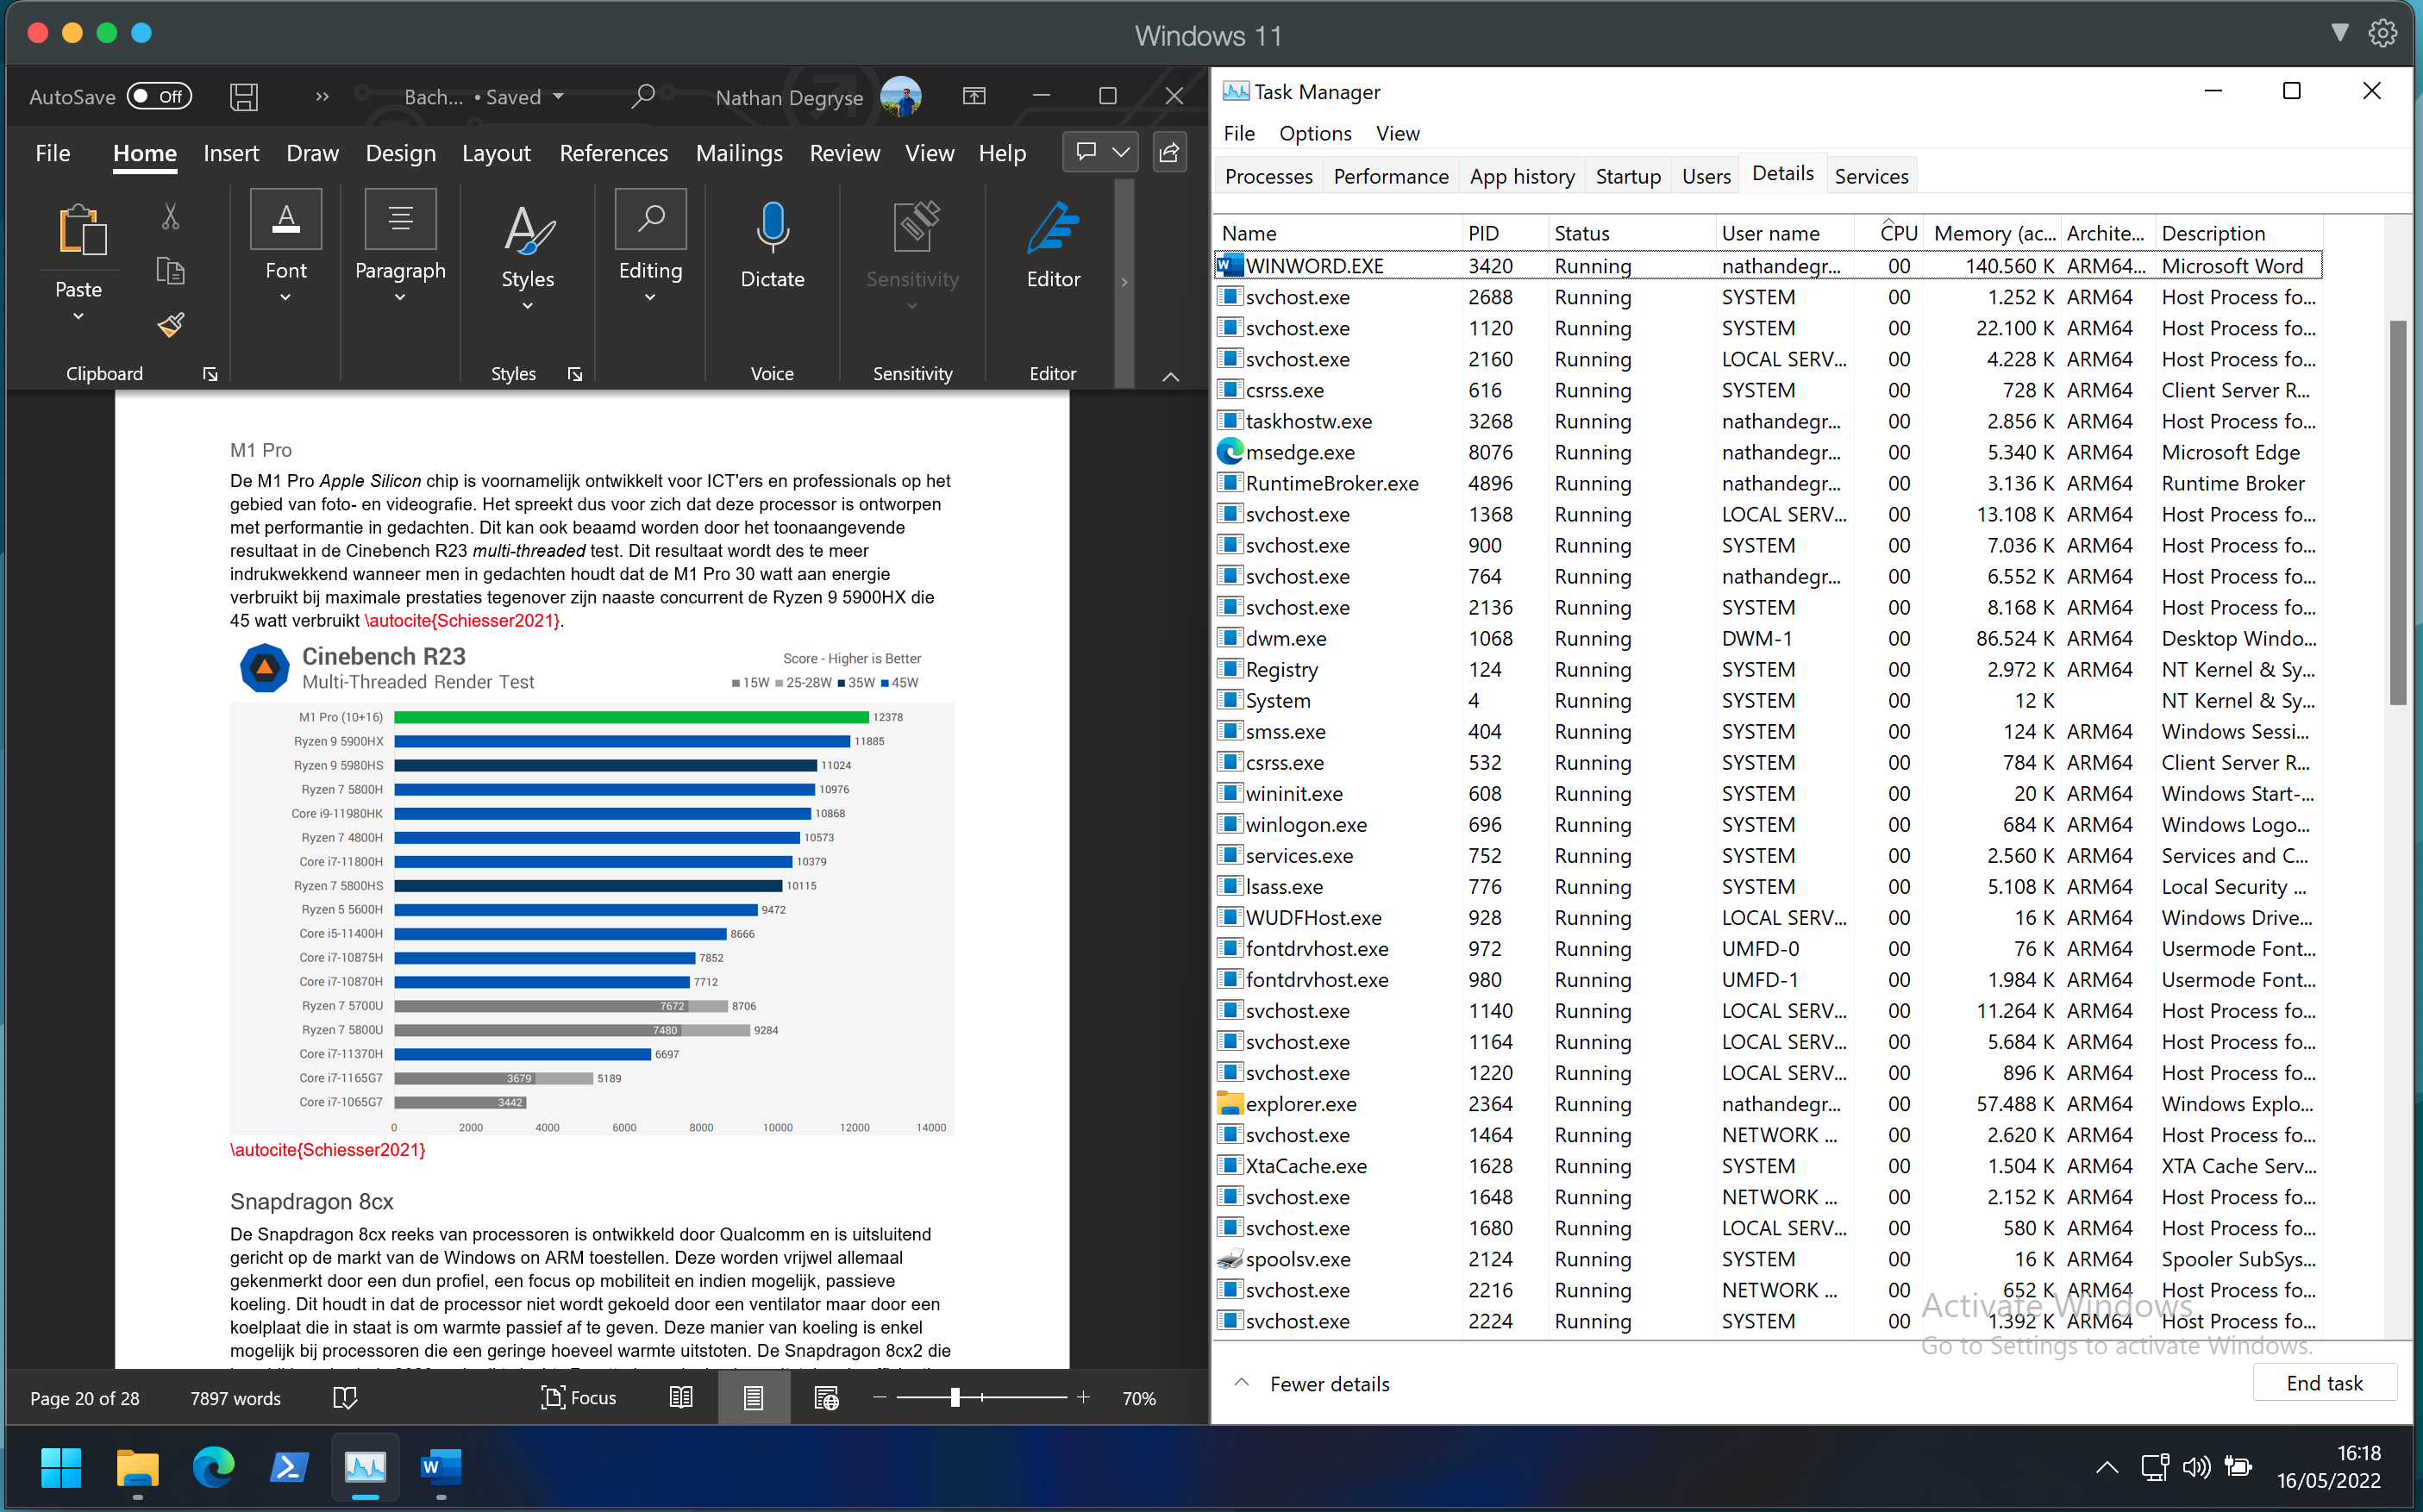
\includegraphics[width=\linewidth]{img/office_winARM.png}
	\caption{Microsoft Office op het Windows on ARM platform}
\end{figure}

Op het gebied van browserondersteuning stelt het Windows on ARM platform enigszins teleur. Microsoft Edge is zoals altijd de standaardbrowser voor Windows toestellen, deze voorziet alle functionaliteit die Microsoft Edge biedt op een x86 systeem. De problemen komen echter opdagen wanneer een gebruiker een andere browser wenst te gebruiken. Google biedt tot op de dag van vandaag geen ARM variant aan van hun marktleidende Chrome webbrowser terwijl Mozilla Firefox en de open source Chromium browser wel vlot verkrijgbaar zijn voor het Windows on ARM platform. Microsoft treft geen blaam voor deze tekortkoming, het voorspelt echter niet veel goeds voor de platformondersteuning wanneer een technologiegigant als Google zijn software niet ter beschikking stelt.

\begin{figure}[!h]
	\centering
	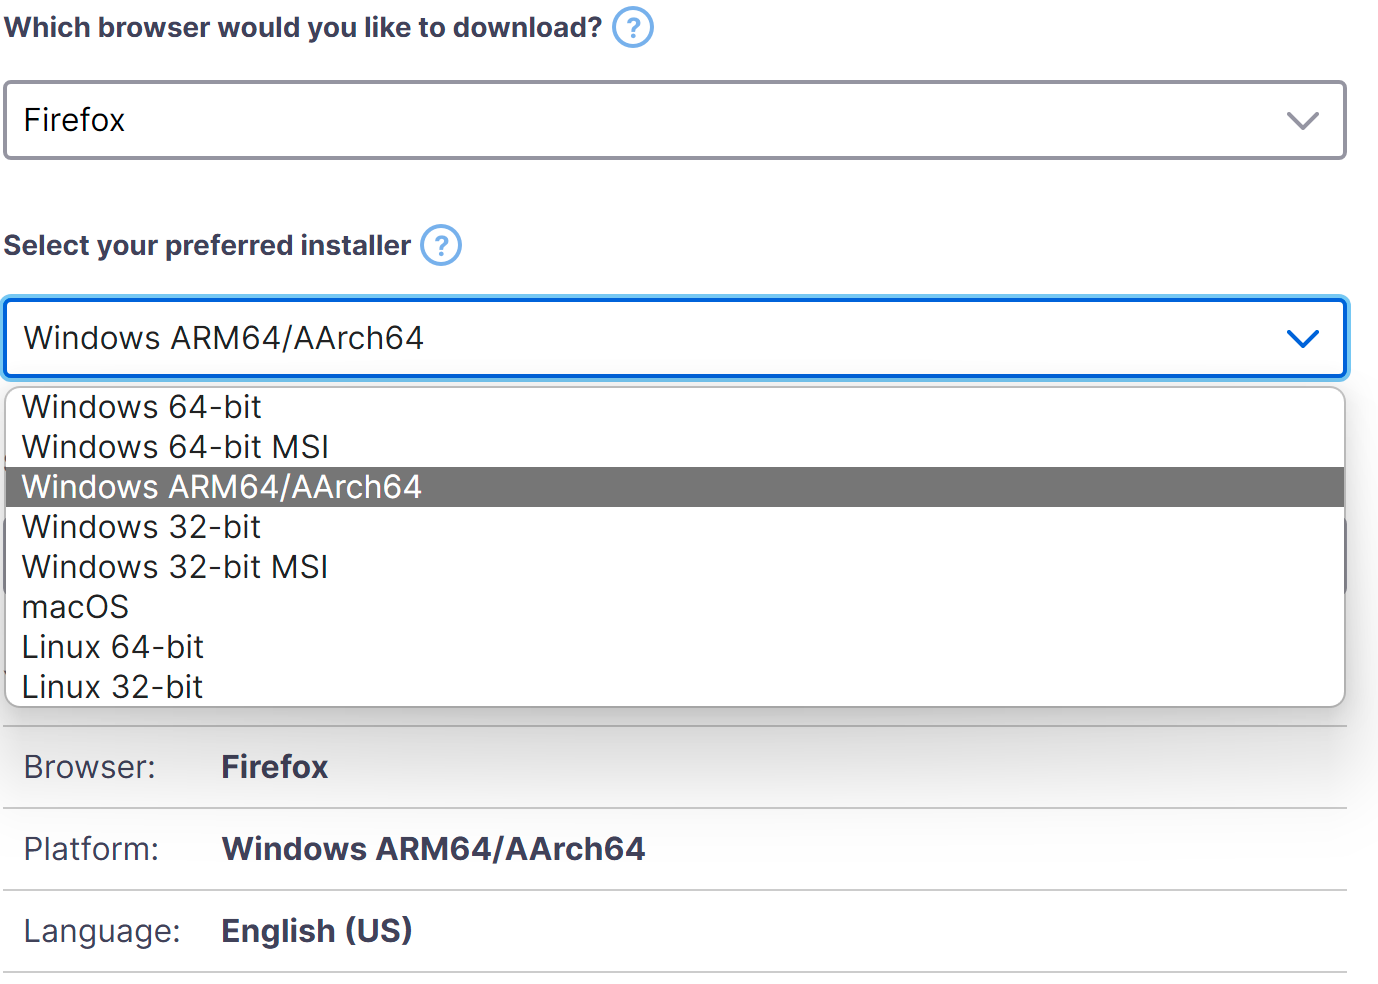
\includegraphics[width=110mm, scale=0.7]{img/firefox_winARM.png}
	\caption{Mozilla Firefox op het Windows on ARM platform \autocite{Mozilla2022}}
\end{figure}

\pagebreak
\section{Scenario 2: professioneel IT-gebruik}
\lipsum[1-4]

\pagebreak
\section{Proof-of-concept Swift applicatie}
Het opzet van deze \textit{proof-of-concept} applicatie is het creëren van een applicatie die uitvoerbaar is op zowel iOS als macOS en dat met een minimum aan overtollige code of verlies aan performantie. Deze opstelling is mogelijk sinds 2020 dankzij de transitie van Intel x86 processoren naar de \textit{Apple Silicon} ARM architectuur \autocite{Apple2020}. Het is tevens belangrijk om te vermelden dat deze platformonafhankelijke manier van applicatie-ontwikkeling enkel mogelijk is op Mac toestellen die gebruik maken van een \textit{Apple Silicon} processor, zijnde de M1, M1 Pro, M1 Max of de M1 Ultra \autocite{AppleDeveloper2022a}. Indien u wenst te controleren of uw toestel gebruik maakt van een \textit{Apple Silicon} processor, dan kan u dit doen via het “Over deze Mac” dialoogvenster. Omwille van privacyredenen is het serienummer in de onderstaande afbeelding onleesbaar gemaakt.

\begin{figure}[h]
    \centering
    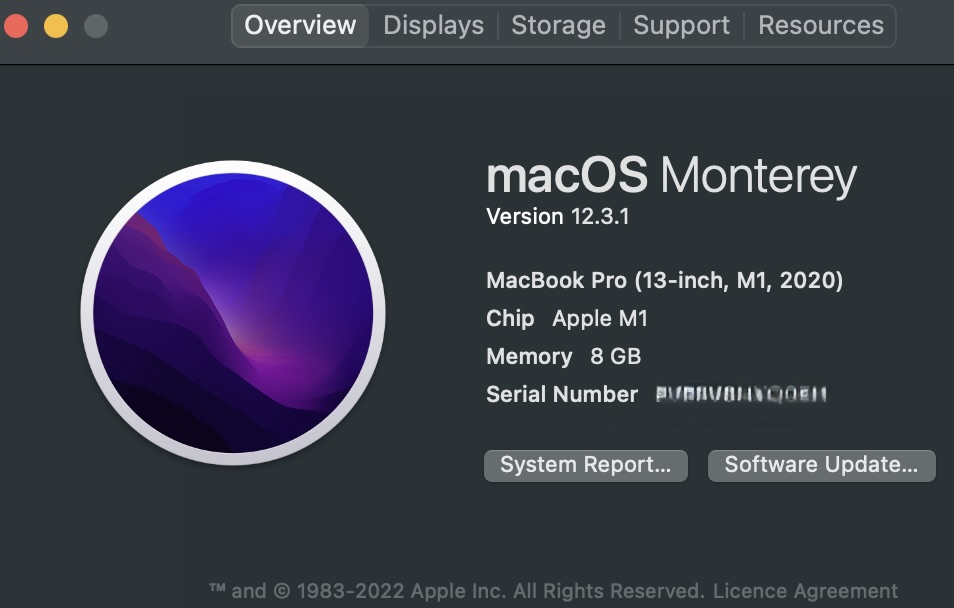
\includegraphics[width=100mm, scale=0.5]{img/overdezemac.jpeg}
    \caption{Het macOS 'Over deze Mac dialoogvenster'}
\end{figure}

De Swift programmeertaal is ontwikkeld door Apple en is reeds in gebruik sinds 2014. Deze wordt gebruikt voor het maken van \textit{native} applicaties voor iOS, iPadOS, macOS, tvOS en watchOS \autocite{AppleDeveloper2022b}. \textit{Native} applicaties worden gecompileerd in de machinetaal van het gekozen hardwareplatform. Vandaar dat applicaties die zijn ontwikkeld voor x86 toestellen niet uitvoerbaar zijn op het ARM platform en vice versa \autocite{Gillis2022}. De Swift taal combineert vaak gebruikte elementen uit de C, Objective C en Python programmeertalen en wordt gekenmerkt door eenvoud en performantie. Er wordt algemeen aangenomen dat Swift applicaties eenvoudiger te ontwikkelen zijn dan hun C en Kotlin tegenhangers omwille van de beginners- en gebruiksvriendelijke syntaxis \autocite{AppleDeveloper2022b}.

Apple voorziet uitstekende handleidingen voor zowel beginners als gevorderden, deze zijn tevens gratis verkrijgbaar in de \textit{Apple Books} online boekenwinkel. Verder stelt Apple een rudimentaire \textit{integrated development environment} (IDE) ter beschikking genaamd Swift Playgrounds. Deze is gericht op beginnende programmeurs of kinderen en jongeren die voor het eerst in aanraking komen met software ontwikkeling. Swift Playgrounds is gratis te verkrijgen op het iPadOS en macOS platform \autocite{AppleDeveloper2022b}.

Xcode is de IDE bij uitstek voor Swift ontwikkelaars aangezien deze een goede balans levert tussen nuttige functies en gebruiksgemak. De bijhorende simulator stelt ontwikkelaars in staat om hun applicaties meteen te testen in een gevirtualiseerde omgeving. Ondersteuning voor de \textit{Apple Silicon} architectuur is inbegrepen in Xcode sinds versie 12. Dit onderzoek maakt gebruik van Xcode 13.3.1 en de bijhorende toepassingen \autocite{AppleDeveloper2022a}.

De \textit{proof-of-concept} applicatie omvat een eenvoudige \textit{hard-coded} nieuwsapplicatie, dit houdt in dat de app niet kan bijgewerkt  worden zonder aanpassingen te maken aan de broncode. Verder maakt de app ook geen gebruik van \textit{API calls}. De focus van dit onderzoek ligt namelijk op het onderzoeken van de compatibiliteit en het gebruiksgemak van de applicatie op meerdere platformen en niet op het ontwikkelen van een geavanceerd programma dat gericht is op consumentengebruik.

Vooraleer een Swift ontwikkelaar wenst te starten met een project, is het aangewezen om te controleren of het besturingssysteem en de IDE gebruikmaken van de meest recente softwareversies. In het geval van macOS is dit uitvoering 12.3.1 en bij Xcode is dit versie 13.3.1.

\begin{figure}[!h]
    \centering
    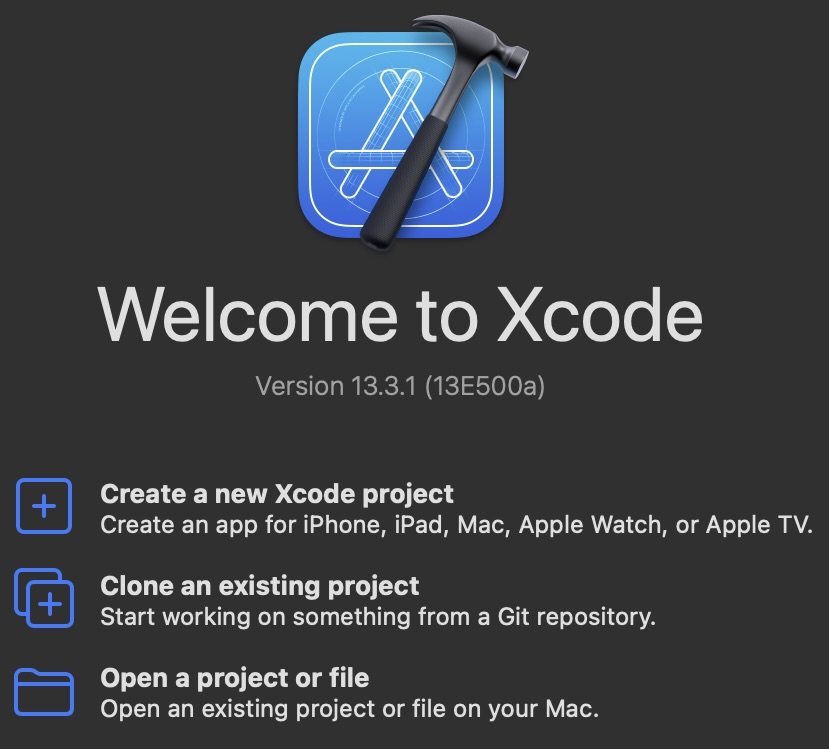
\includegraphics[width=90mm, scale=0.7]{img/xcodeversie.jpeg}
    \caption{Het startscherm van Xcode 13}
\end{figure}

Om te starten met de ontwikkeling van een nieuwe applicatie volstaat het om te kiezen voor de “Create a new Xcode project” optie. Vervolgens verschijnt er een dialoogvenster waar u kan kiezen tussen verschillende sjablonen gaande van iOS applicaties tot programma’s die gericht zijn op het tvOS platform. In het kader van dit onderzoek volstaan de “multiplatform” en “other” sjablonen. Gezien het doel van dit onderzoek, namelijk het onderzoeken van een “multiplatform“ applicatie is, is het aangewezen om te kiezen voor het “other” sjabloon aangezien deze de ontwikkelaar additionele flexibiliteit biedt.

\begin{figure}[!h]
    \centering
    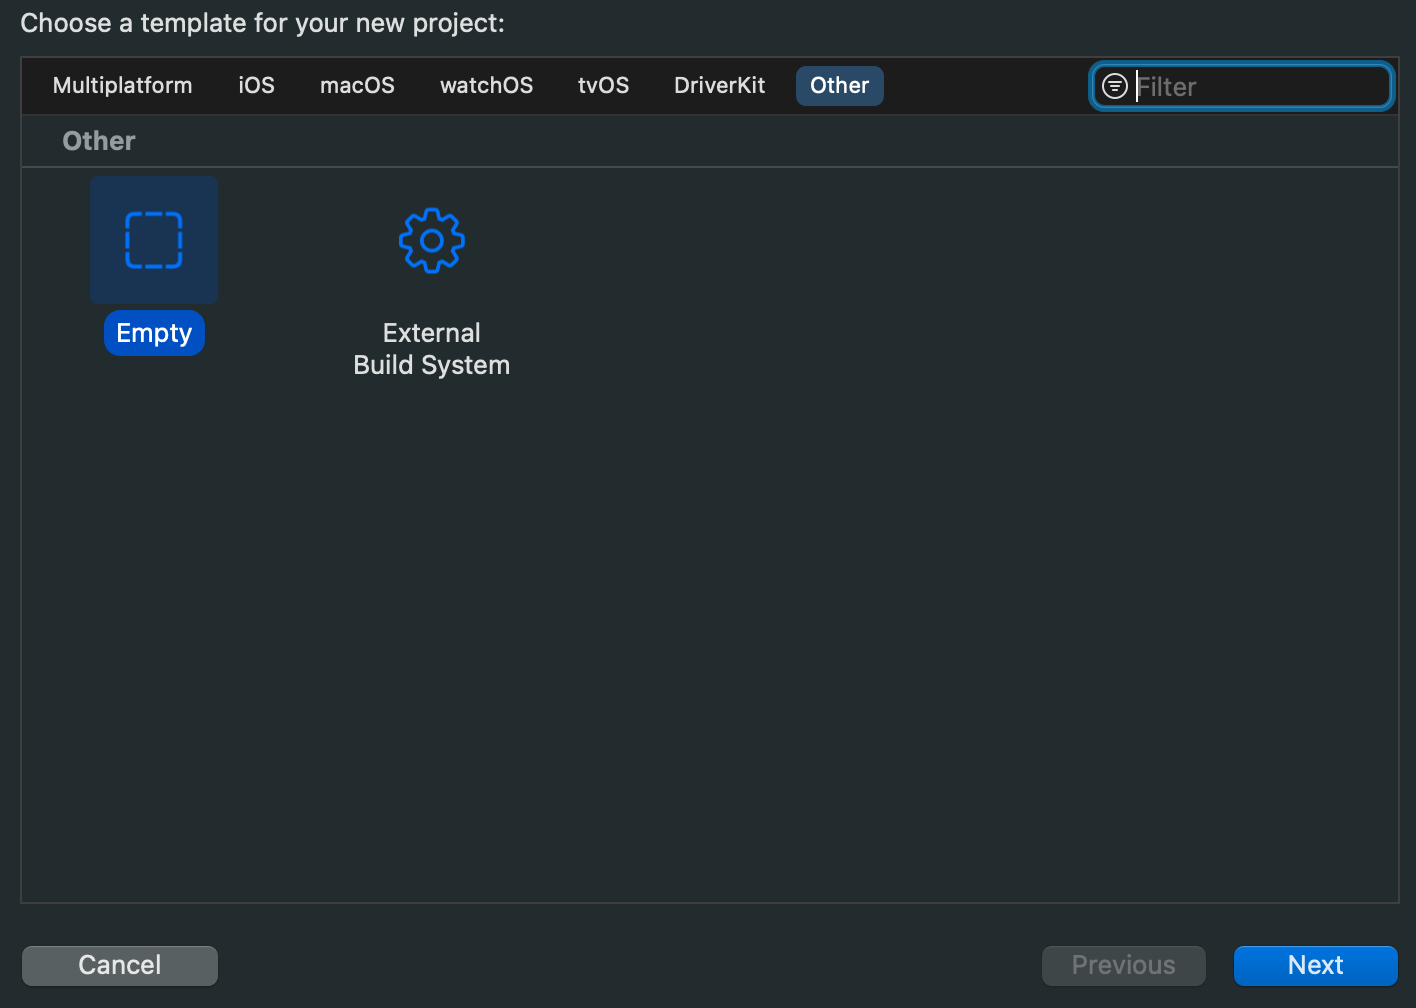
\includegraphics[width=110mm, scale=0.7]{img/otherproject.png}
    \caption{Xcode 13 sjablonen}
\end{figure}

\pagebreak
Na het kiezen van een sjabloon dient een ontwikkelaar een \textit{target} toe te voegen. Een \textit{target} specificeert een te bouwen product en bevat de instructies om dit product te bouwen vanuit een set bestanden in een project- of werkruimte. Een \textit{target} definieert één enkel product, het organiseert de invoer in het bouwsysteem, de bronbestanden en tenslotte de instructies voor het verwerken van de bronbestanden die nodig zijn om het product te bouwen \autocite{AppleDeveloper2011}. Een project kan één of meerdere \textit{targets} bevatten, in het geval van dit project zijn dit macOS en iOS.
\begin{figure}[!h]
    \centering
    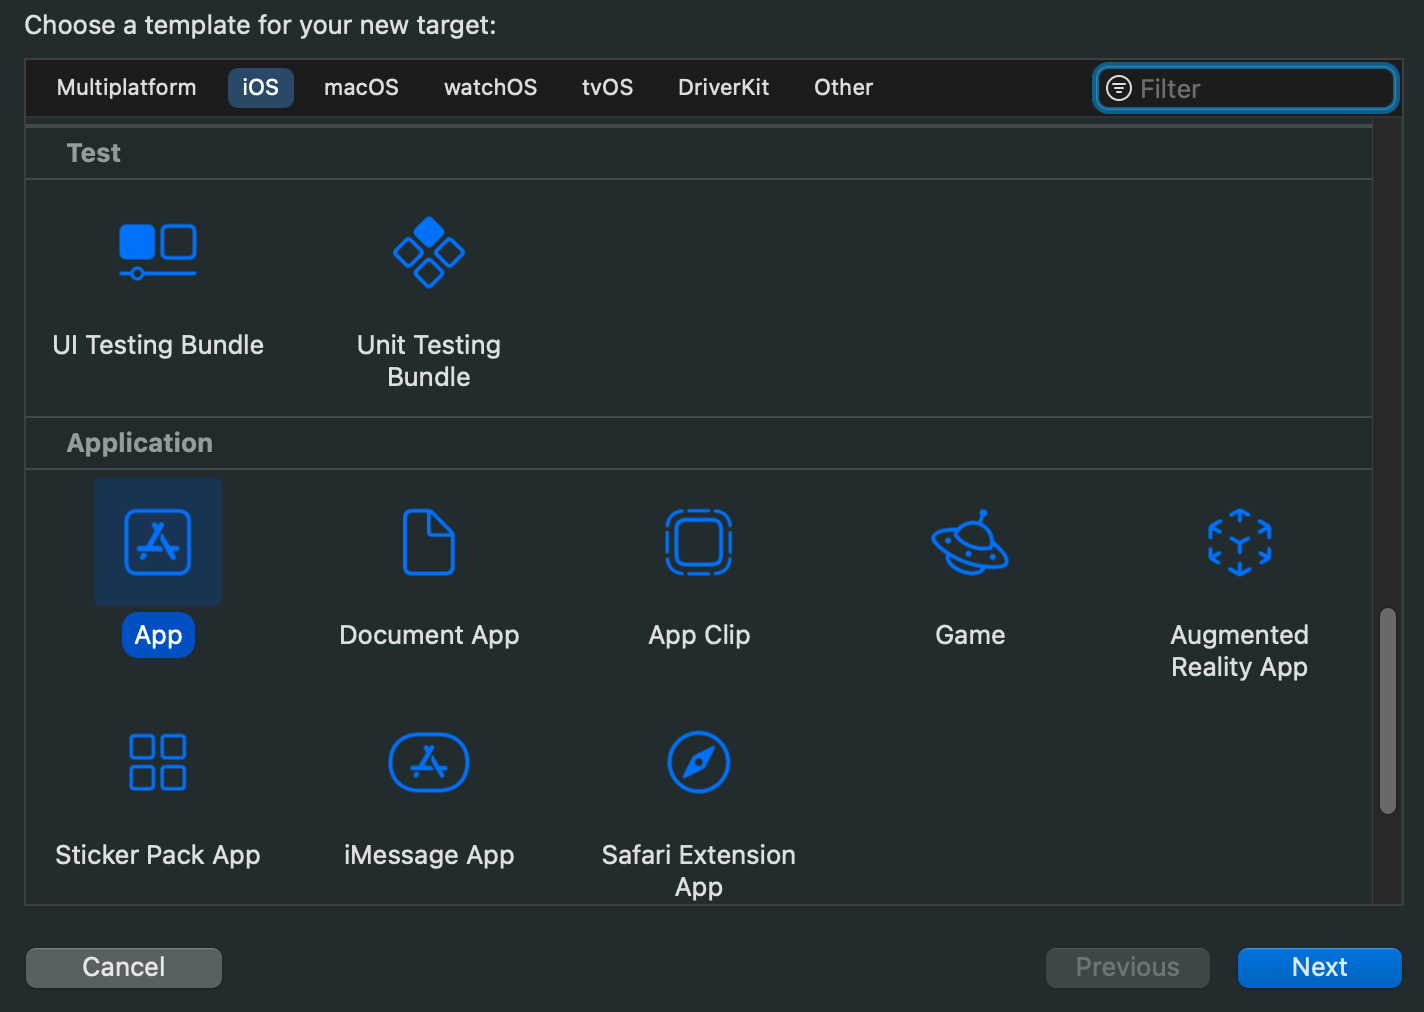
\includegraphics[width=110mm, scale=0.7]{img/iostarget.png}
    \caption{Een overzicht van de verschillende targets}
\end{figure}

\begin{figure}[!h]
    \centering
    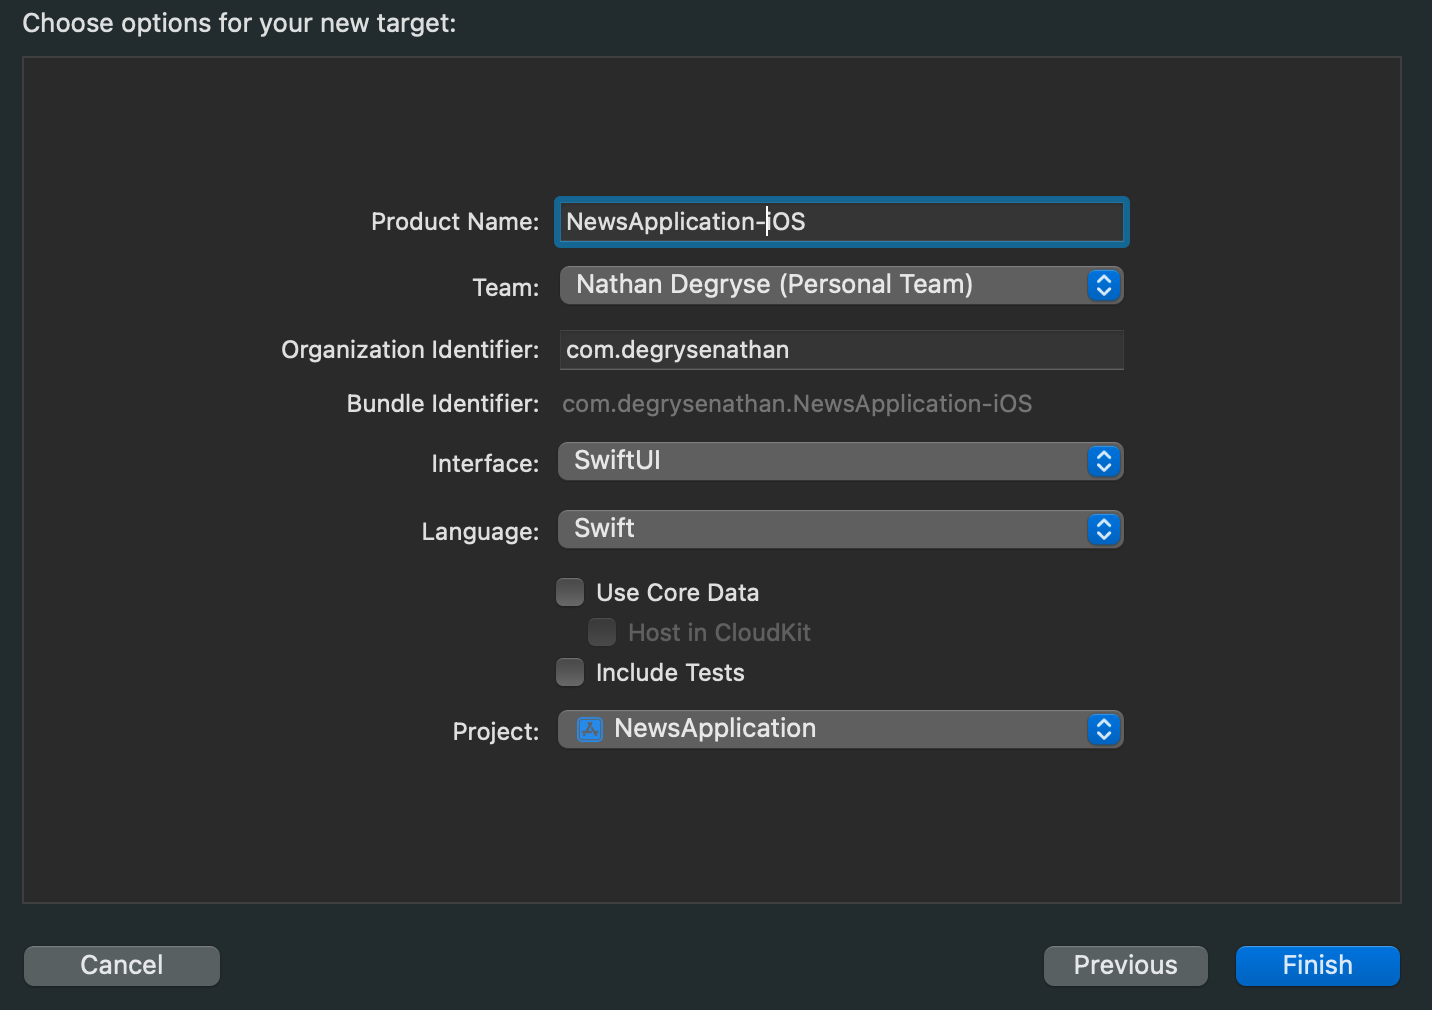
\includegraphics[width=120mm, scale=0.7]{img/iostargetdetail.png}
    \caption{Een detailweergave van het iOS target}
\end{figure}

\newpage
Eenmaal de iOS en macOS \textit{targets} zijn toegevoegd aan het project, is het tijd om een gedeelde \textit{group} aan te maken die in dit geval de naam “shared” heeft gekregen. In deze gedeelde \textit{group} zullen alle \textit{models} en \textit{views} worden opgeslagen. Deze zijn allen toegankelijk vanuit de iOS en macOS targets. De \textit{shared group} kan vervolgens uitgebreid worden met de \textit{models group} waar alle Swift \textit{structures} terechtkomen. \textit{Structures} zijn gelijkaardig aan klassen in andere programmeertalen, maar toch zijn er enkele opmerkelijke verschillen. Een klasse is een \textit{reference type} terwijl een \textit{struct} een \textit{value type} is. Wanneer men een \textit{struct} kopieert, krijgt men twee unieke kopieën van de gegevens. Echter wanneer men een klasse kopieert, verkrijgt men twee verwijzingen naar één instantie van de gegevens \autocite{Khan2021}. De \textit{Article struct} is als volgt opgebouwd: 

\begin{figure}[!h]
    \centering
    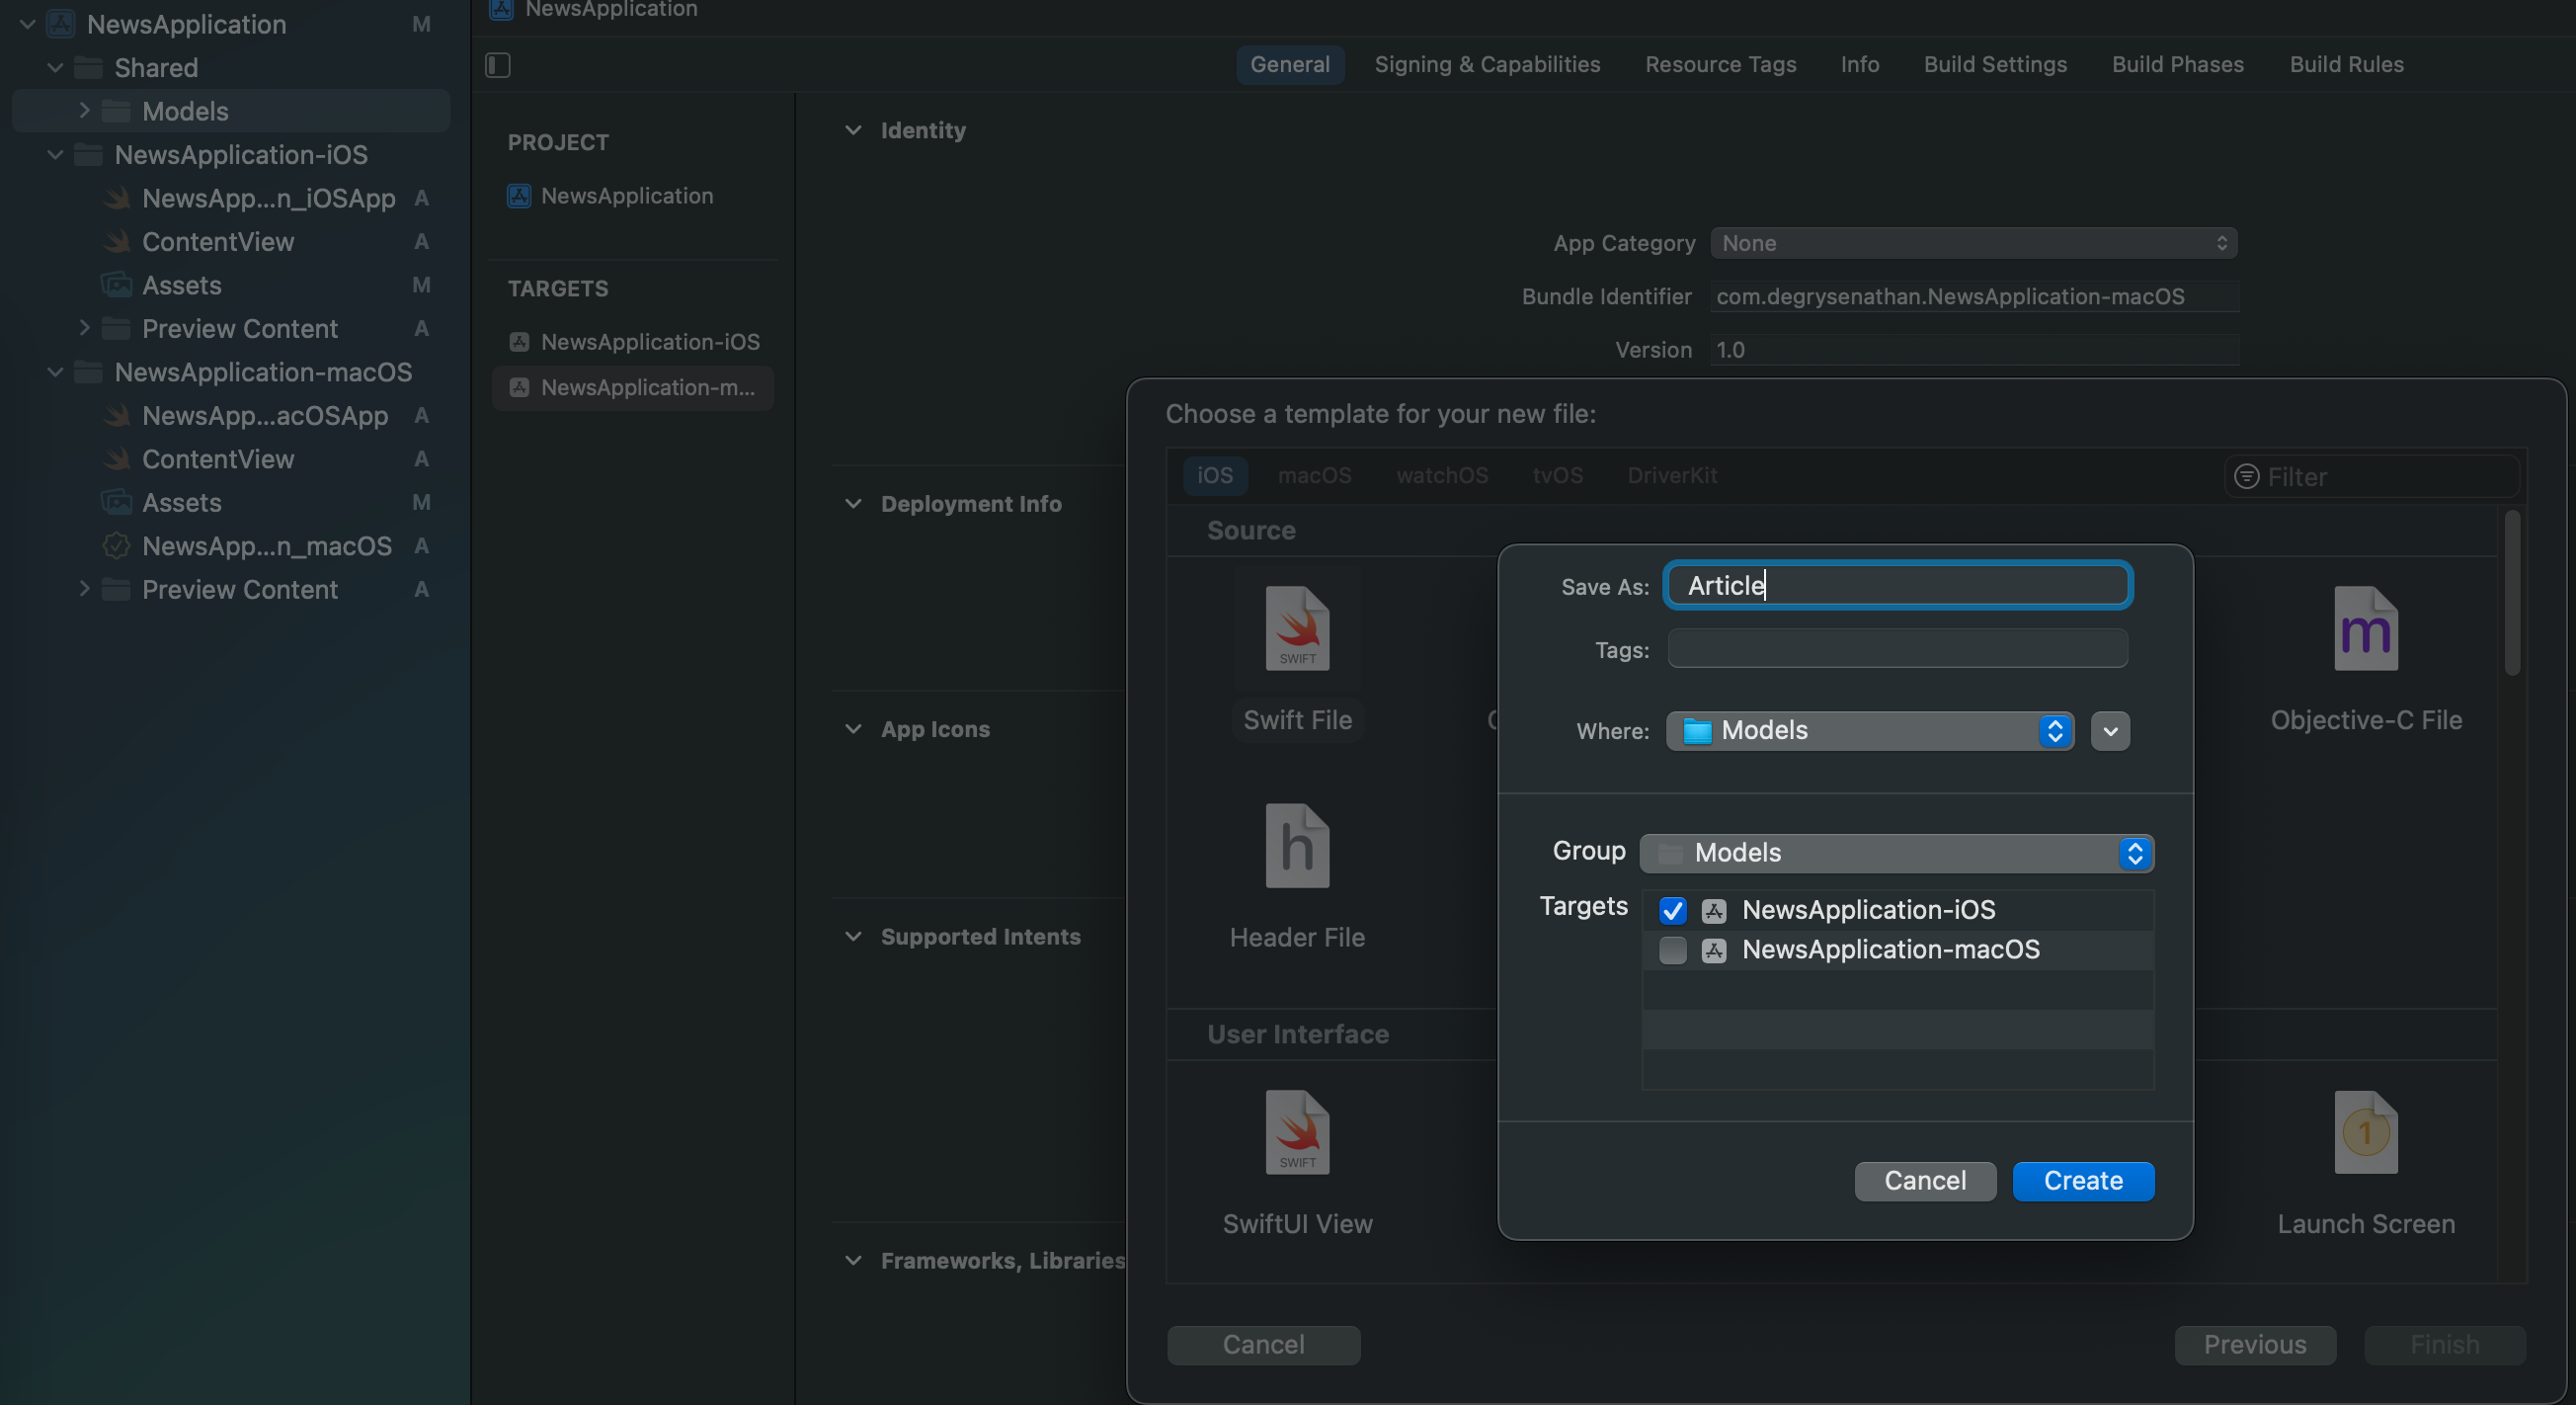
\includegraphics[width=120mm, scale=0.7]{img/articleswift.png}
    \caption{Een overzicht van het initialisatievenster van Article.swift}
\end{figure}

\newpage
\begin{lstlisting}
    
    //  Article.swift
    //  NewsApplication-iOS
    //
    //  Created by Nathan Degryse on 11/05/2022.
    
    import Foundation
    
    enum Subject: String {
        case all = "All"
        case sport = "Sport"
        case internationaal = "Internationaal"
        case regionaal = "Regionaal"
        case politiek = "Politiek"
    }
    
    extension Subject {
        
        var title: String {
            switch self {
                case .all:
                return "All"
                case .sport:
                return "Sport"
                case .internationaal:
                return "Internationaal"
                case .regionaal:
                return "Regionaal"
                case .politiek:
                return "Politiek"
            }
        }
        
    }
    
    struct Article: Identifiable{
        let id = UUID()
        let name: String
        let photo: String
        let description: String
        let rating: Int?
        let subject: Subject
    }
    
\end{lstlisting}
\newpage

Naast de \textit{models group} komt ook de group met alle preview content in de shared group terecht. Apple verwacht dat developers gebruikmaken van SwiftUI \textit{previews}, dit zijn voorvertoningen die live worden bijgewerkt wanneer een ontwikkelaar nieuwe elementen toevoegt of bestaande elementen aanpast/verwijdert. U kunt de standaard asset-catalogus "Preview Assets" gebruiken om voorbeeldafbeeldingen, kleuren en andere soorten assets te configureren die u normaal aan een asset-catalogus zou toevoegen. In dit project wordt de asset-catalogus gebruikt om een voorvertoning te genereren van de afbeeldingen die aan bod zullen komen in de nieuwsartikelen \autocite{VanDerLee2021}. Het is essentieel om aan te geven dat de "Preview Assets" beschikbaar zijn voor beide targets aangezien deze beide gebruik zullen maken van de afbeeldingen.

\begin{figure}[!h]
    \centering
    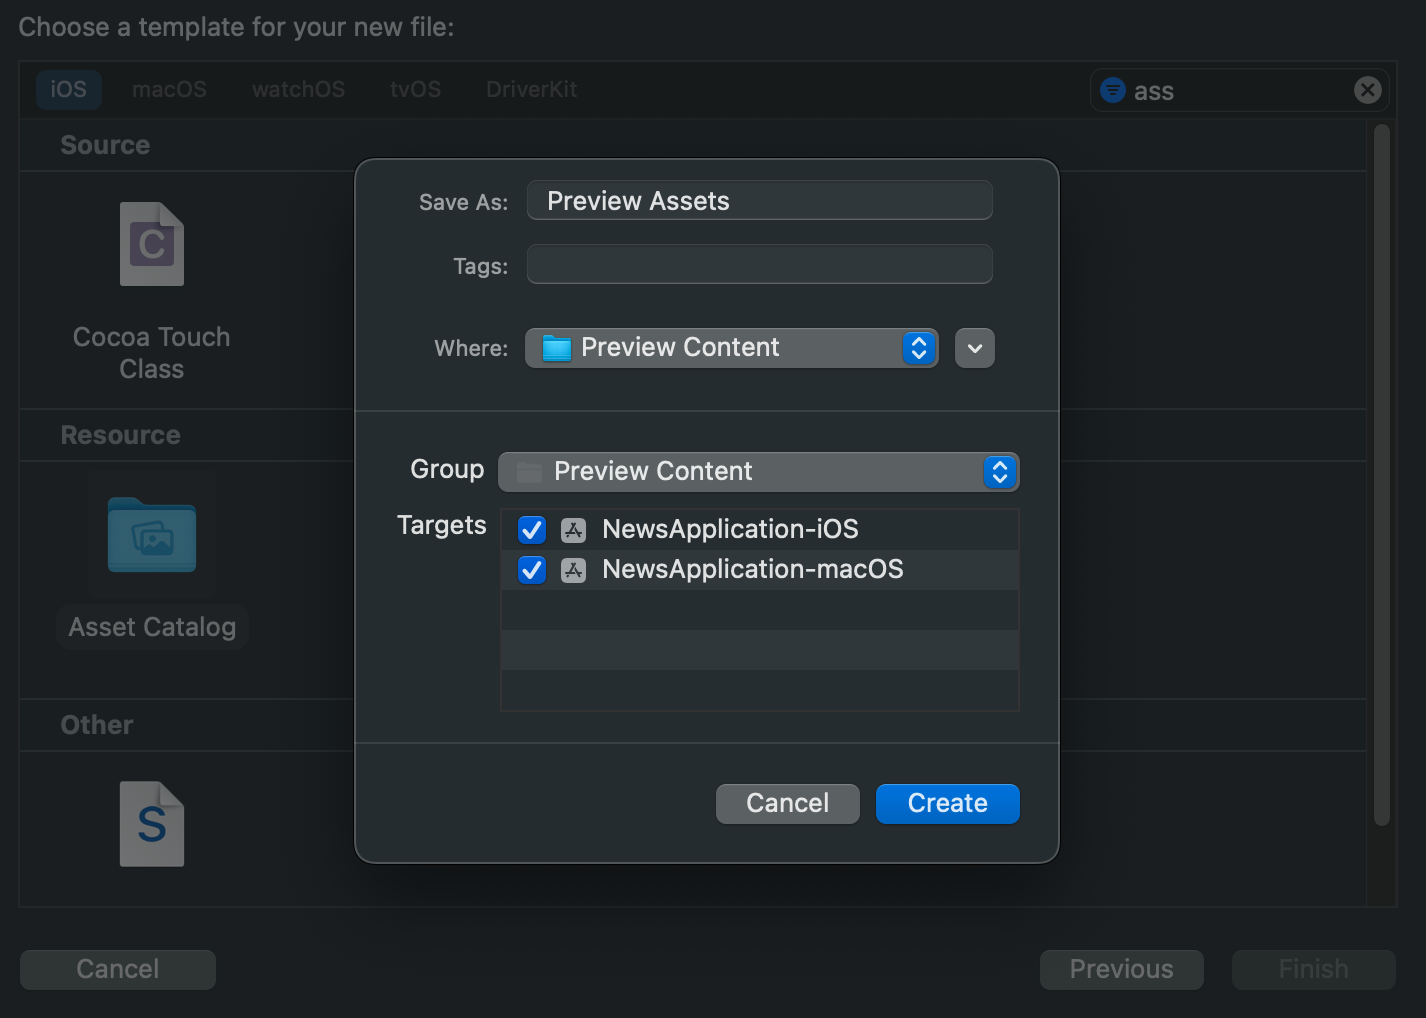
\includegraphics[width=\linewidth]{img/previewassets.png}
    \caption{Een overzicht van het initialisatievenster van de preview assets}
\end{figure}

\pagebreak 
In deze fase van het project is het cruciaal om de \textit{target membership} van de Article.swift file te verifiëren of aan te passen. Deze dient namelijk beschikbaar te zijn voor zowel het iOS- als macOS \textit{target} aangezien beide applicaties gebruik zullen maken van dit bestand.

\begin{figure}[!h]
    \centering
    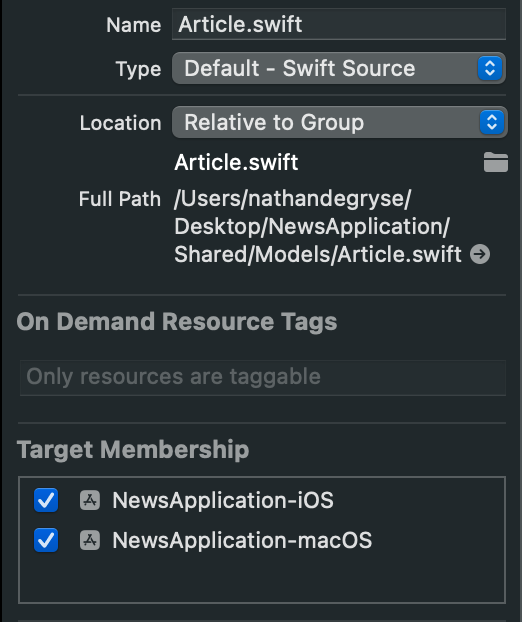
\includegraphics[width=80mm, scale=0.5]{img/articletargetmembership.png}
    \caption{Een overzicht van het targetmembership}
\end{figure}

Tenslotte dient de \textit{views group} ook toegevoegd te worden aan de \textit{shared group}. Deze \textit{group} bestaat uit de volgende \textit{views} die gedeeld moeten worden tussen de verschillende \textit{targets}:

\begin{itemize}
    \item \textbf{ArticleListView:} Deze \textit{view} zal gebruikt worden om een lijstvoorstelling te genereren op basis van alle beschikbare nieuwsartikelen. Deze lijst neemt het volledige scherm in beslag op de iOS applicatie, maar neemt echter slechts een deel van het scherm in beslag op de macOS applicatie. Dit omwille van de extra schermruimte die ter beschikking is op grotere toestellen zoals laptops en desktops.
    \item \textbf{ArticleDetailView:} Deze \textit{view} wordt gebruikt om een detailweergave voor te stellen van het desbetreffende artikel. Op het iOS platform neemt dit het volledige scherm in beslag terwijl dit op het Mac platform slechts een deel confisqueert. 
    \item \textbf{RatingView:} Tenslotte zal deze \textit{view} een grafische voorstelling weergeven van de recensie van het betreffende artikel. 
\end{itemize}

Het is opnieuw essentieel om beide \textit{targets} toe te voegen aan alle \textit{views}.

\pagebreak
Eenmaal alle \textit{views} zijn geïmplementeerd in de gedeelde \textit{group} dient er gerefereerd te worden naar deze vanuit de \textit{target} producten zijnde de iOS en macOS applicaties. In onderstaande afbeelding is te zien hoe dit wordt verwezenlijkt in Swift. Via een \textit{navigation view} kan een gebruiker navigeren doorheen een verzameling binnen een navigatie-gebaseerde applicatie. Gebruikers navigeren naar een weergave door middel van een \textit{NavigationLink} te selecteren die de ontwikkelaar verstrekt. Op iPadOS en macOS verschijnt de inhoud van de bestemming in de volgende beschikbare kolom. Op andere platformen zoals iOS en watchOS wordt een nieuwe weergave op de stapel geplaatst en kunnen items uit de stapel worden verwijderd met platform specifieke besturingselementen, zoals een terug-knop of een veegbeweging \autocite{AppleDeveloper2022c}.

\begin{figure}[!h]
    \centering
    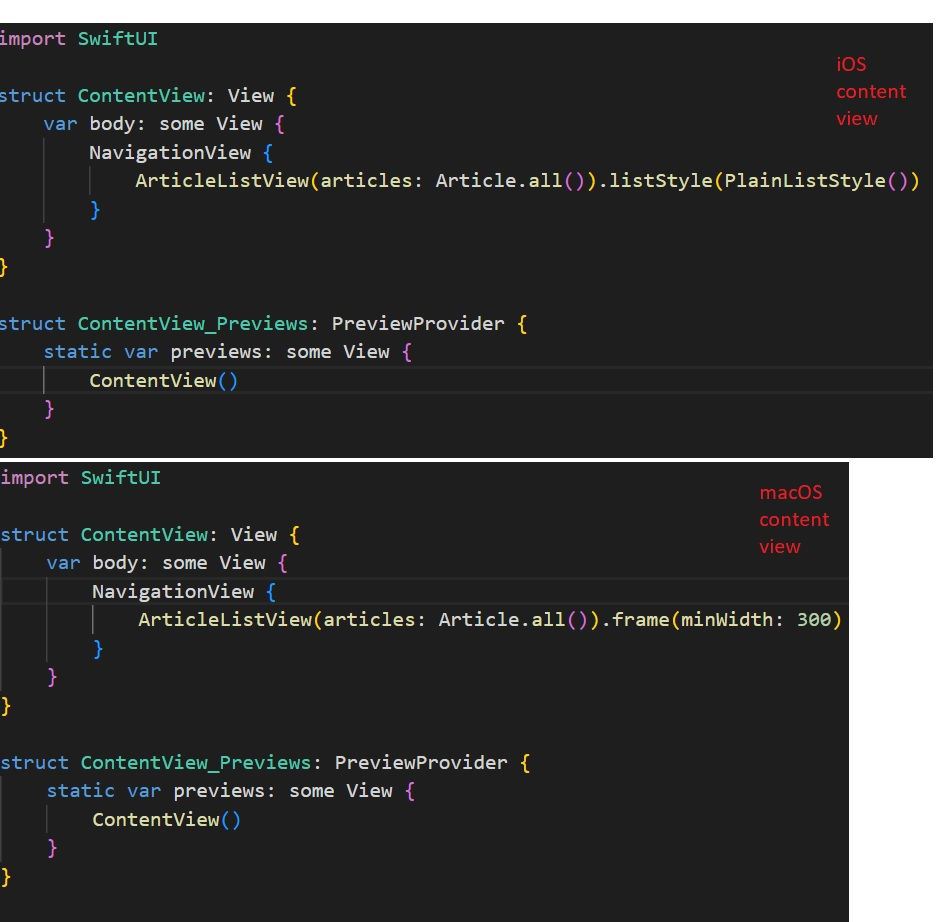
\includegraphics[width=\linewidth]{img/contentview.jpg}
    \caption{Een weergave van de ContentView files}
\end{figure}

\pagebreak
In de onderstaande afbeelding is er tenslotte een overzicht beschikbaar van de finale programmastructuur. Deze omvat de iOS en macOS nieuwsapplicaties die gebruikmaken van de gedeelde \textit{views}, \textit{models} en \textit{preview assets}.

\begin{figure}[!h]
    \centering
    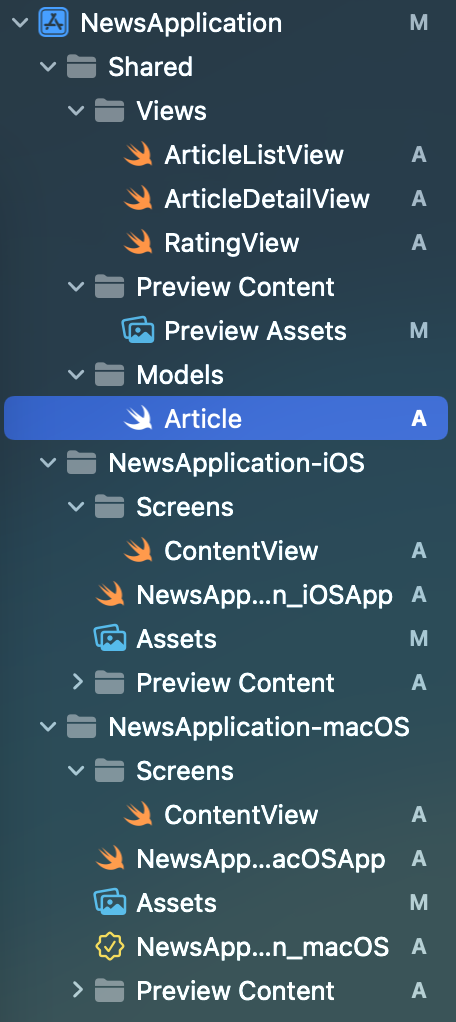
\includegraphics[width=70mm, scale=0.7]{img/applicatiestructuur.png}
    \caption{Een systematisch overzicht van de applicatiestructuur}
\end{figure}

\pagebreak
Deze finale afbeelding biedt een weergave van de iOS en macOS applicaties die simultaan uitvoerbaar zijn. Deze maken gebruik van simulatiesoftware die een onderdeel is van Xcode 13. Nadat een ontwikkelaar een applicatie heeft ontwikkeld, kan deze gecompileerd worden en kan de ontwikkelaar deze uitvoeren en testen op een gesimuleerd of een echt apparaat. Een voordeel van de gesimuleerde aanpak is dat een ontwikkelaar de applicatie kan testen op een uitgebreid gamma van virtuele apparaten gaande van de iPod Touch tot de meest recente iPhone modellen \autocite{AppleDeveloper2021}. De volledige broncode van dit project is beschikbaar via onderstaande URL: \url{https://github.com/DegryseNathan/ARM-van-mobile-naar-desktop/tree/main/NewsApplication}
\\\\
\begin{figure}[!h]
    \centering
    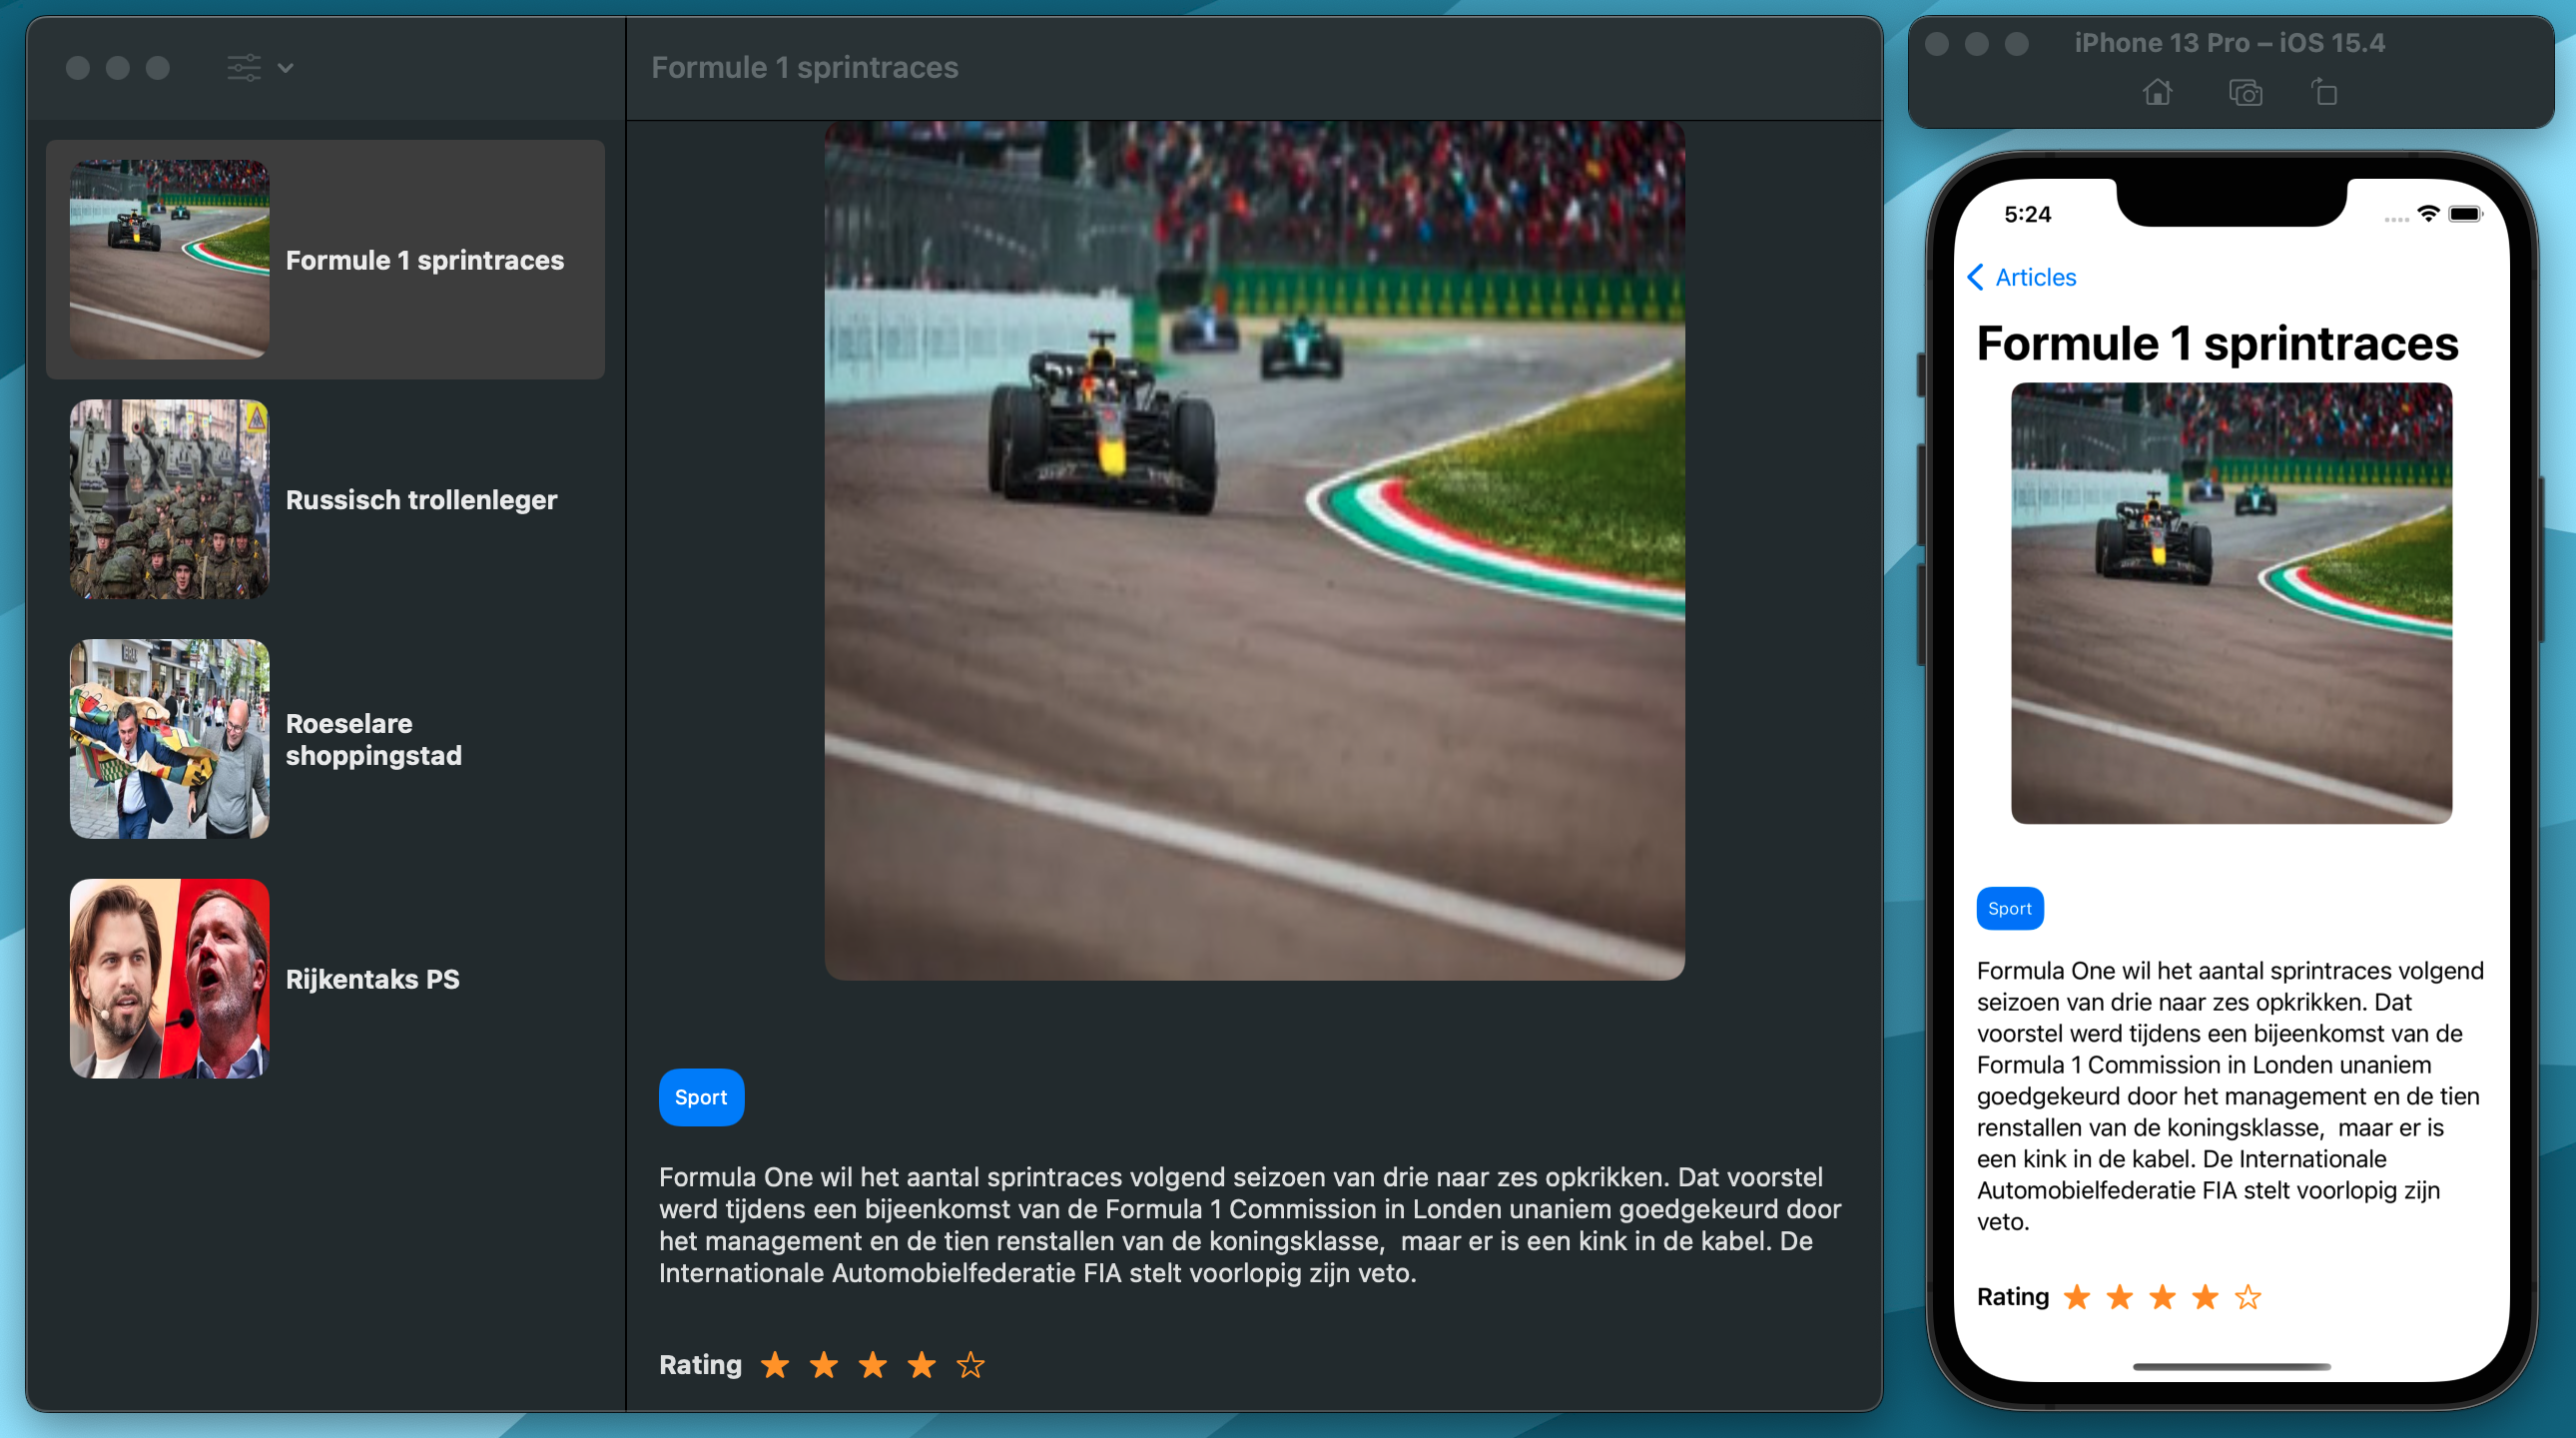
\includegraphics[width=\linewidth]{img/iosenmacosapplicatie.png}
    \caption{Een overzicht van de iOS en macOS nieuwsapplicatie}
\end{figure}
